\documentclass[10pt,journal,compsoc]{IEEEtran}

% *** CITATION PACKAGES ***
%
\ifCLASSOPTIONcompsoc
  % IEEE Computer Society needs nocompress option
  % requires cite.sty v4.0 or later (November 2003)
  \usepackage[nocompress]{cite}
\else
  % normal IEEE
  \usepackage{cite}
\fi

\usepackage{booktabs} % For formal tables
\usepackage[utf8]{inputenc}
\usepackage[english]{babel}
\usepackage[T1]{fontenc}
\usepackage{url}
\usepackage{graphicx}
\usepackage{graphics}
\usepackage{listings}  
\usepackage{array}
\newcolumntype{L}[1]{>{\raggedright\let\newline\\\arraybackslash\hspace{0pt}}m{#1}}
\newcolumntype{C}[1]{>{\centering\let\newline\\\arraybackslash\hspace{0pt}}m{#1}}
\newcolumntype{R}[1]{>{\raggedleft\let\newline\\\arraybackslash\hspace{0pt}}m{#1}}
\usepackage{multirow}
%\usepackage[table]{xcolor}
\usepackage{float}
\usepackage{array}
\usepackage{ragged2e}
\usepackage{subcaption}
\usepackage{tikz}
\usepackage[normalem]{ulem}
\usepackage{amsmath}
\usepackage{mathpazo}
\usepackage{amsfonts}
\usepackage{framed}
\usepackage{cleveref}

\newcolumntype{P}[1]{>{\RaggedRight\hspace{0pt}}p{#1}}

\lstset{language=Java,
	tabsize=2,
	basicstyle=\ttfamily\footnotesize,
	mathescape=true
} 

\newenvironment{boxquote}{\vspace{-1ex}\setlength{\FrameSep}{1\fboxsep}\begin{framed}\setlength{\parskip}{0.5\baselineskip}\setlength{\parindent}{0pt}}{\end{framed}}

\newcommand{\squeezeup}{\vspace{-0.5mm}}

\usepackage{etoolbox}
\makeatletter
\patchcmd{\@makecaption}
{\scshape}
{}
{}
{}
\makeatother

\newcolumntype{"}{@{\hskip\tabcolsep\vrule width 1pt\hskip\tabcolsep}}

\newcommand\FIXME[1]{{\color{red}\textbf{FIXME: #1}}}

% correct bad hyphenation here
%\hyphenation{op-tical net-works semi-conduc-tor}

\begin{document}

\title{Toxic Code Snippets on Stack Overflow}

\author{Chaiyong Ragkhitwetsagul,~Jens Krinke,~Matheus Paixao,~Giuseppe Bianco,~Rocco Oliveto}

% The paper headers
\markboth{IEEE TRANSACTIONS ON SOFTWARE ENGINEERING,~Vol.~X, No.~Y, Month~2018}%
{Ragkhitwetsagul \MakeLowercase{\textit{et al.}}: Toxic Code Snippets on Stack Overflow}
% The only time the second header will appear is for the odd numbered pages
% after the title page when using the twoside option.
% 
% *** Note that you probably will NOT want to include the author's ***
% *** name in the headers of peer review papers.                   ***
% You can use \ifCLASSOPTIONpeerreview for conditional compilation here if
% you desire.

% The publisher's ID mark at the bottom of the page is less important with
% Computer Society journal papers as those publications place the marks
% outside of the main text columns and, therefore, unlike regular IEEE
% journals, the available text space is not reduced by their presence.
% If you want to put a publisher's ID mark on the page you can do it like
% this:
%\IEEEpubid{0000--0000/00\$00.00~\copyright~2015 IEEE}
% or like this to get the Computer Society new two part style.
%\IEEEpubid{\makebox[\columnwidth]{\hfill 0000--0000/00/\$00.00~\copyright~2015 IEEE}%
%\hspace{\columnsep}\makebox[\columnwidth]{Published by the IEEE Computer Society\hfill}}
% Remember, if you use this you must call \IEEEpubidadjcol in the second
% column for its text to clear the IEEEpubid mark (Computer Society jorunal
% papers don't need this extra clearance.)

% for Computer Society papers, we must declare the abstract and index terms
% PRIOR to the title within the \IEEEtitleabstractindextext IEEEtran
% command as these need to go into the title area created by \maketitle.
% As a general rule, do not put math, special symbols or citations
% in the abstract or keywords.
\IEEEtitleabstractindextext{%
\begin{abstract}
Online code clones are code fragments that are copied from software projects or
online sources to Stack Overflow as examples. Due to an absence of a checking
mechanism after the code has been copied to Stack Overflow, they can become
toxic code snippets, e.g.,~they suffer from being outdated or violating the
original software license. We present a study of online code clones on Stack
Overflow and their toxicity by incorporating two developer surveys and a
large-scale code clone detection. A survey of 201 high-reputation Stack Overflow
answerers (33\% response rate) showed that 131 participants (65\%) have ever
been notified of outdated code and 26 of them (20\%) rarely or never fix the
code. 138 answerers (69\%) never check for licensing conflicts between their
copied code snippets and Stack Overflow's CC BY-SA 3.0. A survey of 87 Stack
Overflow visitors shows that they experienced several issues from Stack Overflow
answers: mismatched solutions, outdated solutions, incorrect solutions, and buggy code. 
85\% of them are not aware of CC BY-SA 3.0
license enforced by Stack Overflow, and 66\% never check for license conflicts
when reusing code snippets. Our clone detection found online clone pairs between
72,365 Java code snippets on Stack Overflow and 111 open source projects in the
curated Qualitas corpus. We analysed 2,289 non-trivial online clone candidates.
Our investigation revealed strong evidence that 153 clones have been copied from
a Qualitas project to Stack Overflow. We found 100 of them (66\%) to be outdated,  
of which 10 were buggy and harmful for reuse.
Furthermore, we found 214 code snippets that
could potentially violate the license of their original software and appear 7,112
times in 2,427 GitHub projects.

%Online code clones are code fragments that are copied from software projects or
%online sources to Stack Overflow as examples in questions and answers. % They
%Due to an absence of a checking mechanism after the code has been copied to
%Stack Overflow, they can become toxic code snippets, i.e.~they suffer from
%being outdated or violating the original software license. We present a study
%incorporating several state-of-the-art tools and techniques to automatically
%extract and filter detected online clone pairs between 72,365 Java code snippets
%on Stack Overflow and 111 Java open source projects in the curated Qualitas
%corpus. We discovered and analysed 2,289 non-trivial online clone candidates.
%Our investigation of the online clone pairs revealed strong evidence that 154
%clones have been copied from a Qualitas project to Stack Overflow.  We found 101
%of them (66\%) to be outdated and potentially harmful for reuse.  Furthermore,
%we found 214 code snippets on Stack Overflow that could potentially violate the license of their
%original software. To better understand the phenomenon, we also surveyed 201 high-reputation Stack Overflow answerers
%(33\% response rate) and found that 131 of the answerers (65\%) have ever been notified of
%outdated code in the answers and 26 of them (20\%) rarely or never fix the outdated
%code. Only 3 answerers explicitly include software licenses in their answers and
%138 answerers (69\%) never check for licensing conflicts between their copied code
%snippets and Stack Overflow's CC BY-SA 3.0.
\end{abstract}

% Note that keywords are not normally used for peerreview papers.
\begin{IEEEkeywords}
Code Clone Detection, Stack Overflow, Outdated Code, Software Licensing
\end{IEEEkeywords}}


% make the title area
\maketitle


% To allow for easy dual compilation without having to reenter the
% abstract/keywords data, the \IEEEtitleabstractindextext text will
% not be used in maketitle, but will appear (i.e., to be "transported")
% here as \IEEEdisplaynontitleabstractindextext when the compsoc 
% or transmag modes are not selected <OR> if conference mode is selected 
% - because all conference papers position the abstract like regular
% papers do.
\IEEEdisplaynontitleabstractindextext
% \IEEEdisplaynontitleabstractindextext has no effect when using
% compsoc or transmag under a non-conference mode.



% For peer review papers, you can put extra information on the cover
% page as needed:
% \ifCLASSOPTIONpeerreview
% \begin{center} \bfseries EDICS Category: 3-BBND \end{center}
% \fi
%
% For peerreview papers, this IEEEtran command inserts a page break and
% creates the second title. It will be ignored for other modes.
\IEEEpeerreviewmaketitle

\IEEEraisesectionheading{\section{Introduction}\label{sec:introduction}}

%The popularity of the Internet encourages tremendous amount of source code
% being shared online.
Stack Overflow is a popular online programming community with 7.6 million users,
14 million questions, and 23 million answers\footnote{Data as of 21 August 2017
	from~\url{https://stackexchange.com/sites}}. It allows programmers to ask
questions and give answers to programming problems. The website has found to be
useful for software
development~\cite{Ponzanelli2013,Ponzanelli2014,Keivanloo2014,Park2014,
	Stolee2014,Subramanian2013,Diamantopoulos2015,Treude2016} and also valuable for
educational purposes~\cite{Nasehi2012}. On Stack Overflow, each conversation
contains a question and a list of answers. The answers frequently contain at
least one code snippet as a solution to the question asked. We found that the
code snippets are often not authored directly on the Stack Overflow website
but copied from another location. A snippet in an answer could be copied and
modified from a code snippet in the question, copied from the answerer's own
code or from other locations including open source software (OSS) systems.

The process of posting and answering questions on Stack Overflow that involves
the reuse (copying) of source code can be considered code cloning. Code cloning
is an activity of reusing source code by copying and pasting. It normally occurs
in software development and account from 7\% to 23\% of source code in typical
software systems~\cite{Bellon2007}. The benefits and drawbacks of clones are
still controversial. Several authors state that clones lead to bug propagations
and software maintenance issues~\cite{Kamiya2002}, while some others suggest
that clones are not harmful and can even be
beneficial~\cite{Saini2016,Kapser2006}.

Code cloning can also have side effects such as violating software licenses or
introducing software vulnerabilities. Carelessly cloning code from one project
to another project with a different license may cause a software license
violation~\cite{German2009}. This also happens within the context of online Q\&A
websites such as Stack Overflow. An et al.~\cite{An2017} showed that 1,279
cloned snippets between Android apps and Stack Overflow potentially violate
software licenses. Security is also among the main concerns when the code is copied
from an online source. For example, Stack Overflow helps developers to solve
Android programming problems more quickly than other resources while, at the
same time, offers less secure code than books or the official Android
documentation~\cite{Acar2016}.

\begin{figure*}
  \fboxsep0pt
	\begin{lstlisting}[escapechar=&]
/* Code in Stack Overflow post ID 22315734 */         /* WritableComparator.java (2014-11-21) */
public int compare(byte[] b1,int s1,int l1, ...) {    public int compare(byte[] b1,int s1,int l1, ...) {
  try {                                                 try {
    buffer.reset(b1,s1,l1); /* parse key1 */              buffer.reset(b1,s1,l1); /* parse key1 */
    key1.readFields(buffer);                              key1.readFields(buffer);
    buffer.reset(b2,s2,l2); /* parse key2 */              buffer.reset(b2,s2,l2); /* parse key2 */
    key2.readFields(buffer);                              key2.readFields(buffer);
  } catch (IOException e) {                               &\framebox{buffer.reset(null,0,0); \textit{/* clean up reference */}}&
    throw new RuntimeException(e);                      } catch (IOException e) {
  }                                                       throw new RuntimeException(e);
  return compare(key1,key2); /* compare them */         }
}                                                       return compare(key1, key2); /* compare them */
                                                      }
	\end{lstlisting}\vspace{-2ex}
	\caption{An example of the two code fragments of
		{\small\texttt{WritableComparator.java}}. The one from the
		Stack Overflow post 22315734 (left) is outdated when compared to
		its latest version in the \textsf{Hadoop} code base
		(right). Its Apache v.2.0 license is also missing.}
	\label{fig:before-after}
\end{figure*}

We call code snippets that are copied from software systems to online Q\&A
websites (such as Stack Overflow) and vice versa as ``online code clones.''
There are two directions in creating online code clones: (1)~code is cloned from
a software project to a Q\&A website as an example; or (2)~code is cloned from a
Q\&A website to a software project to obtain a functionality, perform a
particular task, or fixing a bug. % and (3)~code is transferred from one
% software project to another via a Q\&A website;
Similar to classic code clones, i.e.,~clones between software systems, online
code clones can lead to license violations, bug propagation, an introduction of
vulnerabilities, and re-use of outdated code. Unfortunately, online clones are
difficult to locate and fix since the search space in online code corpora is
larger and no longer confined to a local repository.

To have a deeper insight into online code clones, we surveyed 201 high-reputation
Stack Overflow answerers. The results of such a survey show that online code
cloning occurs on Stack Overflow. Stack Overflow answerers frequently clone code
from other locations, such as their personal projects, company projects, and
open source projects, to Stack Overflow as a solution or a complement to a
solution. The code cloning activity on Stack Overflow is obviously beneficial
considered the popularity of Stack Overflow and its influence on software
development~\cite{Ponzanelli2013,Ponzanelli2014,Park2014}. On the other hand,
there is also a downside caused by low quality, defective, and harmful code
snippets that are reused without awareness by millions of users~\cite{Zhang2018,Acar2016,Fischer2017}.

One participant in our survey expresses his/her concerns about this:

\begin{quote}
	\textit{``The real issue is less about the amount the code snippets
	on SO than it is about the staggeringly high number of software
	``professionals'' that mindlessly use them without understanding what they're
	copying, and the only slightly less high number of would-be professionals that
	post snippets with built-in security issues.  A related topic is beginners who
	post (at times dangerously) misleading tutorials online on topics they actually
	know very little about. Think PHP/MySQL tutorials written 10+ years after
	\texttt{mysql\_*} functions were obsolete, or the recent regex tutorial that
	got posted the other day on HackerNew
	(\url{https://news.ycombinator.com/item?id=14846506}). They're also full of
	toxic code snippets.''}
\end{quote}

Although this activity of online code cloning is well-known, there are only a few
empirical studies on the topic~\cite{An2017,Abdalkareem2017,Baltes2017}, especially
on finding the origins of the clones on Q\&A websites.
In this study, we tackle this challenge of establishing the existence of online code 
clones on Stack Overflow, investigate how they occur, and study the potential
effects to software reusing them.
%Using the same analogy, in this study, we are interested in 
Therefore, we mine Stack Overflow posts, detected online code clones, and analysed the clones to reveal
``toxic code snippets.''

Toxic code snippets mean code snippets that, after incorporating into software, degrade the software quality.
Stack Overflow code snippets
cloned from open source software or online sources can become toxic when they
are (1)~outdated, (2)~violating their original software
license, (3)~exhibiting code smells, (4)~containing faults, or (5)~having security vulnerabilities.
In this study, we focus on the first two forms of toxic code snippets, outdated code and license-violating code,
as these two problems are still underexplored compared to code smells~\cite{Tufano2015} and vulnerabilities~\cite{Acar2016,Fischer2017}.
Moreover, Stack Overflow users also express their concerns about these two problems
as shown in several discussion threads\footnote{Discussions about outdated answers and code license on
	Stack Overflow: meta.stackexchange.com/questions/131495, 
	meta.stackexchange.com/questions/11705/, meta.stackexchange.com/questions/12527,
	meta.stackexchange.com/questions/25956, meta.stackoverflow.com/questions/321291.}
	 on \textsf{meta.stackexchange.com} about outdated
answers and license of code on Stack Overflow.
Outdated code snippets can be harmful since they are not up-to-date with their originals and may
contain defects. Code snippets from open source projects usually fall under a
specific software license, e.g.,\ GNU General Public License (GPL). If they are
cloned to Stack Overflow answers without the license, and then flow to other projects
with conflicting licenses, legal issues may occur.

We would like to motivate the readers by giving two examples of toxic code
snippets. The first example is an outdated and potentially license-violating
online code clone in an answer to a Stack Overflow question regarding how to
implement {\small{\texttt{RawComparator}}} in
\textsf{Hadoop}\footnote{\url{http://stackoverflow.com/questions/22315734}}.
\Cref{fig:before-after} shows---on the left---a code snippet embedded as a part
of the accepted answer. The snippet shows how \textsf{Hadoop} implements the
{\small{\texttt{compare}}} method in its {\small{\texttt{WritableComparator}}}
class. The code snippet on the right shows another version of the same method,
but at this time extracted from the latest version (as of October 3, 2017) of
\textsf{Hadoop}. We can see that they both are highly similar except a line
containing {\small{\verb|buffer.reset(null,0,0);|}} which was added on November
21, 2014. The added line is intended for cleaning up the reference in the
{\small{\verb|buffer|}} variable and avoid excess heap usage (issue
no.~HADOOP-11323\footnote{https://issues.apache.org/jira/browse/HADOOP-11323}).
While this change has already been introduced into the
{\small{\texttt{compare}}} method several years ago, the code example in Stack
Overflow post is still unchanged. %This example shows that inconsistencies
%between online code clones and their originals can lead users of Stack Overflow
%to reuse outdated code.
In addition, the original code snippet of {\small\texttt{WritableComparator}}
class in Hadoop is distributed with Apache license version 2.0 while its cloned
instance on Stack Overflow contains only the {\small{\texttt{compare}}} method
and ignores its license statement on top of the file. There are two potential
issues for this. First, the code snippet may appear to be under Stack Overflow's
CC BY-SA 3.0 instead of its original Apache license. Second, if the code snippet
is copied and incorporated into another software project with a conflicting
license, a legal issue may arise.

\begin{figure*}
	\begin{lstlisting}
/* Code in Stack Overflow post ID 801987 */            /* StringUtils.java (2013-02-05) */
public static String humanReadableInt(long number) {   public static String humanReadableInt(long number) {
  long absNumber = Math.abs(number);                     return TraditionalBinaryPrefix.long2String(number,"",1);
  double result = number;                              }
  String suffix = "";
  if (absNumber < 1024) {
  } else if (absNumber < 1024 * 1024) {
    result = number / 1024.0;
    suffix = "k";
  } else if (absNumber < 1024 * 1024 * 1024) {
    result = number / (1024.0 * 1024);
    suffix = "m";
  } else {
    result = number / (1024.0 * 1024 * 1024);
    suffix = "g";
  }
  return oneDecimal.format(result) + suffix;
}
	\end{lstlisting}\vspace{-2ex}
	\caption{An example of the two code fragments of
		{\small\texttt{StringUtils.java}}. The one from the
		Stack Overflow post 801987 (left) is outdated when compared to
		its latest version in the \textsf{Hadoop} code base
		(right). The toxic code snippet is outdated code and has race conditions.}
	\label{fig:before-after_2}
\end{figure*}

The second motivating example of outdated online code clones with more
disrupting changes than the first one  can be found in an answer to a Stack
Overflow question regarding how to format files sizes in a human-readable form.
\Cref{fig:before-after_2} shows---on the left---a code snippet to perform the
task from the {\small{\texttt{StringUtils}}} class in \textsf{Hadoop}. The code snippet on the
right shows another version of the same method, but at this time extracted from
the latest version of \textsf{Hadoop}. We can see that
they are entirely different. The {\small{\texttt{humanReadableInt}}} method is
rewritten on February 5, 2013 to solve an issue of a race condition
(issue no.~HADOOP-9252\footnote{https://issues.apache.org/jira/browse/HADOOP-9252}).
%Similar to the first example, the clone code snippet on Stack Overflow does not 
%include its original Apache v.2.0 license.

The two toxic code snippets in our examples have been posted on March 11, 2014 and
April 9, 2009 respectively. They have already been viewed 259 and 2,886 times\footnote{The number of views
is for the whole Stack Overflow post but we use it as a proxy of the number of views the accepted answer receives
because the question and the answer of the two motivation examples have a short gap of posting time (within the same day and four days after).} 
at
the time of writing this paper (October 3, 2017). Our calculation finds that
there will be a new viewer of the first toxic snippet approximately every 5
days compared to almost every day for the second one. 
%A quick web search shows
%that the defective {\small{\texttt{humanReadableInt}}} method in the second
%example already appears in approximately 500 projects on GitHub. 
Considering the popularity of Stack Overflow, which has more than 50 million developers visiting
each month\footnote{Data as of 21 August 2017 from:
	\url{https://stackoverflow.com}}, one toxic code snippet on Stack Overflow can
spread and grow to hundred or thousand copies within only a year or two.

%The code snippet on Stack Overflow can be outdated. %Since reusing source code from Stack Overflow is considered a common practice nowadays, the scale of online code cloning is more than intra or inter project clone in a local code bases.
%This is an emerging and challenging problem. Since studies in this area are still limited, we aim to gain more insight of the problem in this study. %We are interested to gain more insights of online code clone in this study.

While research has mostly focused on reusing code snippets \emph{from} Stack
Overflow (e.g.,~\cite{Keivanloo2014,An2017,Yang2016}), fewer studies have been
conducted on finding the origins of code examples copied \emph{to} Stack
Overflow and the awareness of Stack Overflow developers in doing so. Finding the
origins of code examples reveals the problem of toxic code snippets
caused by outdated code and software licensing violations. It is equally
important to studying the effects of reusing Stack Overflow code snippets
because it gives insights into the root cause of the problem and lays a
foundation to an automatic technique to detect and report
toxic code snippets on Stack Overflow to developers in the future.

This paper makes the following primary contributions:

\begin{enumerate} 
	
	\item \textbf{Awareness of Stack Overflow answerers and visitors to toxic code
	snippets:} We performed an online survey and collected answers from 201
highly-ranked Stack Overflow users and 87 Stack Overflow visitors. 
We found that the answerers cloned code snippets
from open source projects to Stack Overflow answers. While Stack Overflow
answerers are aware of their outdated code snippets, 19\% of the participants
rarely or never fix the code. 99\% of the answerers never include a software
license in their snippets and 69\% never check for licensing conflicts.
On the other hand, 66\% of the
Stack Overflow visitors experienced problems from reusing Stack Overflow code snippets, including outdated code. 
They are generally not aware of the CC BY-SA 3.0 license, and more than
half of them never check for license compatibility when reusing Stack Overflow
code snippets.
	
	\item \textbf{A manual study of online code clones:} 
	To empirically confirm the findings from the surveys, we used
	two clone detection tools to discover 2,289 similar code snippet pairs between
	72,365 Java code snippets obtained from Stack Overflow's accepted answers and
	111 Java open source projects from the curated Qualitas
	corpus~\cite{QualitasCorpus}. We manually
	classified all of them.
	
	\item \textbf{An investigation of toxic code snippets on Stack Overflow:} Our study shows that from
	the 2,289 online clones, at least 328 have been copied from open source
	projects or external online sources to Stack Overflow, potentially violating
	software licenses. For 153 of them, we found evidence that they have been copied
	from a specific open source project. 
	100 of them were found to be outdated, of which 10 were buggy code.
	
	\item \textbf{An online code
		clone oracle:} The 2,289 manually investigated and validated online clone pairs
	are available for download\footnote{https://ucl-crest.github.io/cloverflow-web} and
	can be used as a clone oracle. \end{enumerate}

\section{Empirical Study}

We performed an empirical study of online code clones between Stack
Overflow and 111 Java open source projects to answer the following
research questions:
\begin{itemize}
	
	\item \textbf{RQ1 (Stack Overflow answerers' and visitors' awareness to toxic code snippets): }
	
	\textit{1)~How often are Stack Overflow
		answerers aware of the outdated code and licensing conflicts when
		they answer a question on Stack Overflow?} 
	
	\textit{2) How often do Stack Overflow
		visitors experience the outdated code and licensing conflicts when
		they reuse code in an answer from Stack Overflow?} 
	
	We surveyed 201 high-reputation Stack Overflow answerers and 87 Stack Overflow visitors to study their
	awareness of the two issues.

	\item \textbf{RQ2 (Online code clones): }\textit{To what extent is source
		code cloned between Stack Overflow and open source projects?} We
	quantitatively measured the number of online code clones between Stack
	Overflow and open source projects to understand the scale of the
	problem. 
	
	\item \textbf{RQ3 (Patterns of online code clones): }\textit{How do online
		code clones occur?} We categorised online clones into seven
	categories allowing insights into how online code clones are created.
	
	\item \textbf{RQ4 (Outdated online code clones): }\textit{Are
		online code clones up-to-date compared to their counterparts in the
		original projects?} We were interested in the outdated Stack
	Overflow code examples since users are potentially reusing
	them. 
	
	\item \textbf{RQ5 (Software licensing violation): }\textit{How often do
		license conflicts occur between Stack Overflow clones and their
		originals?} We investigated whether the reuse of online code clones
	can cause software developers to violate licenses.
\end{itemize}

\begin{figure}
	\centering
	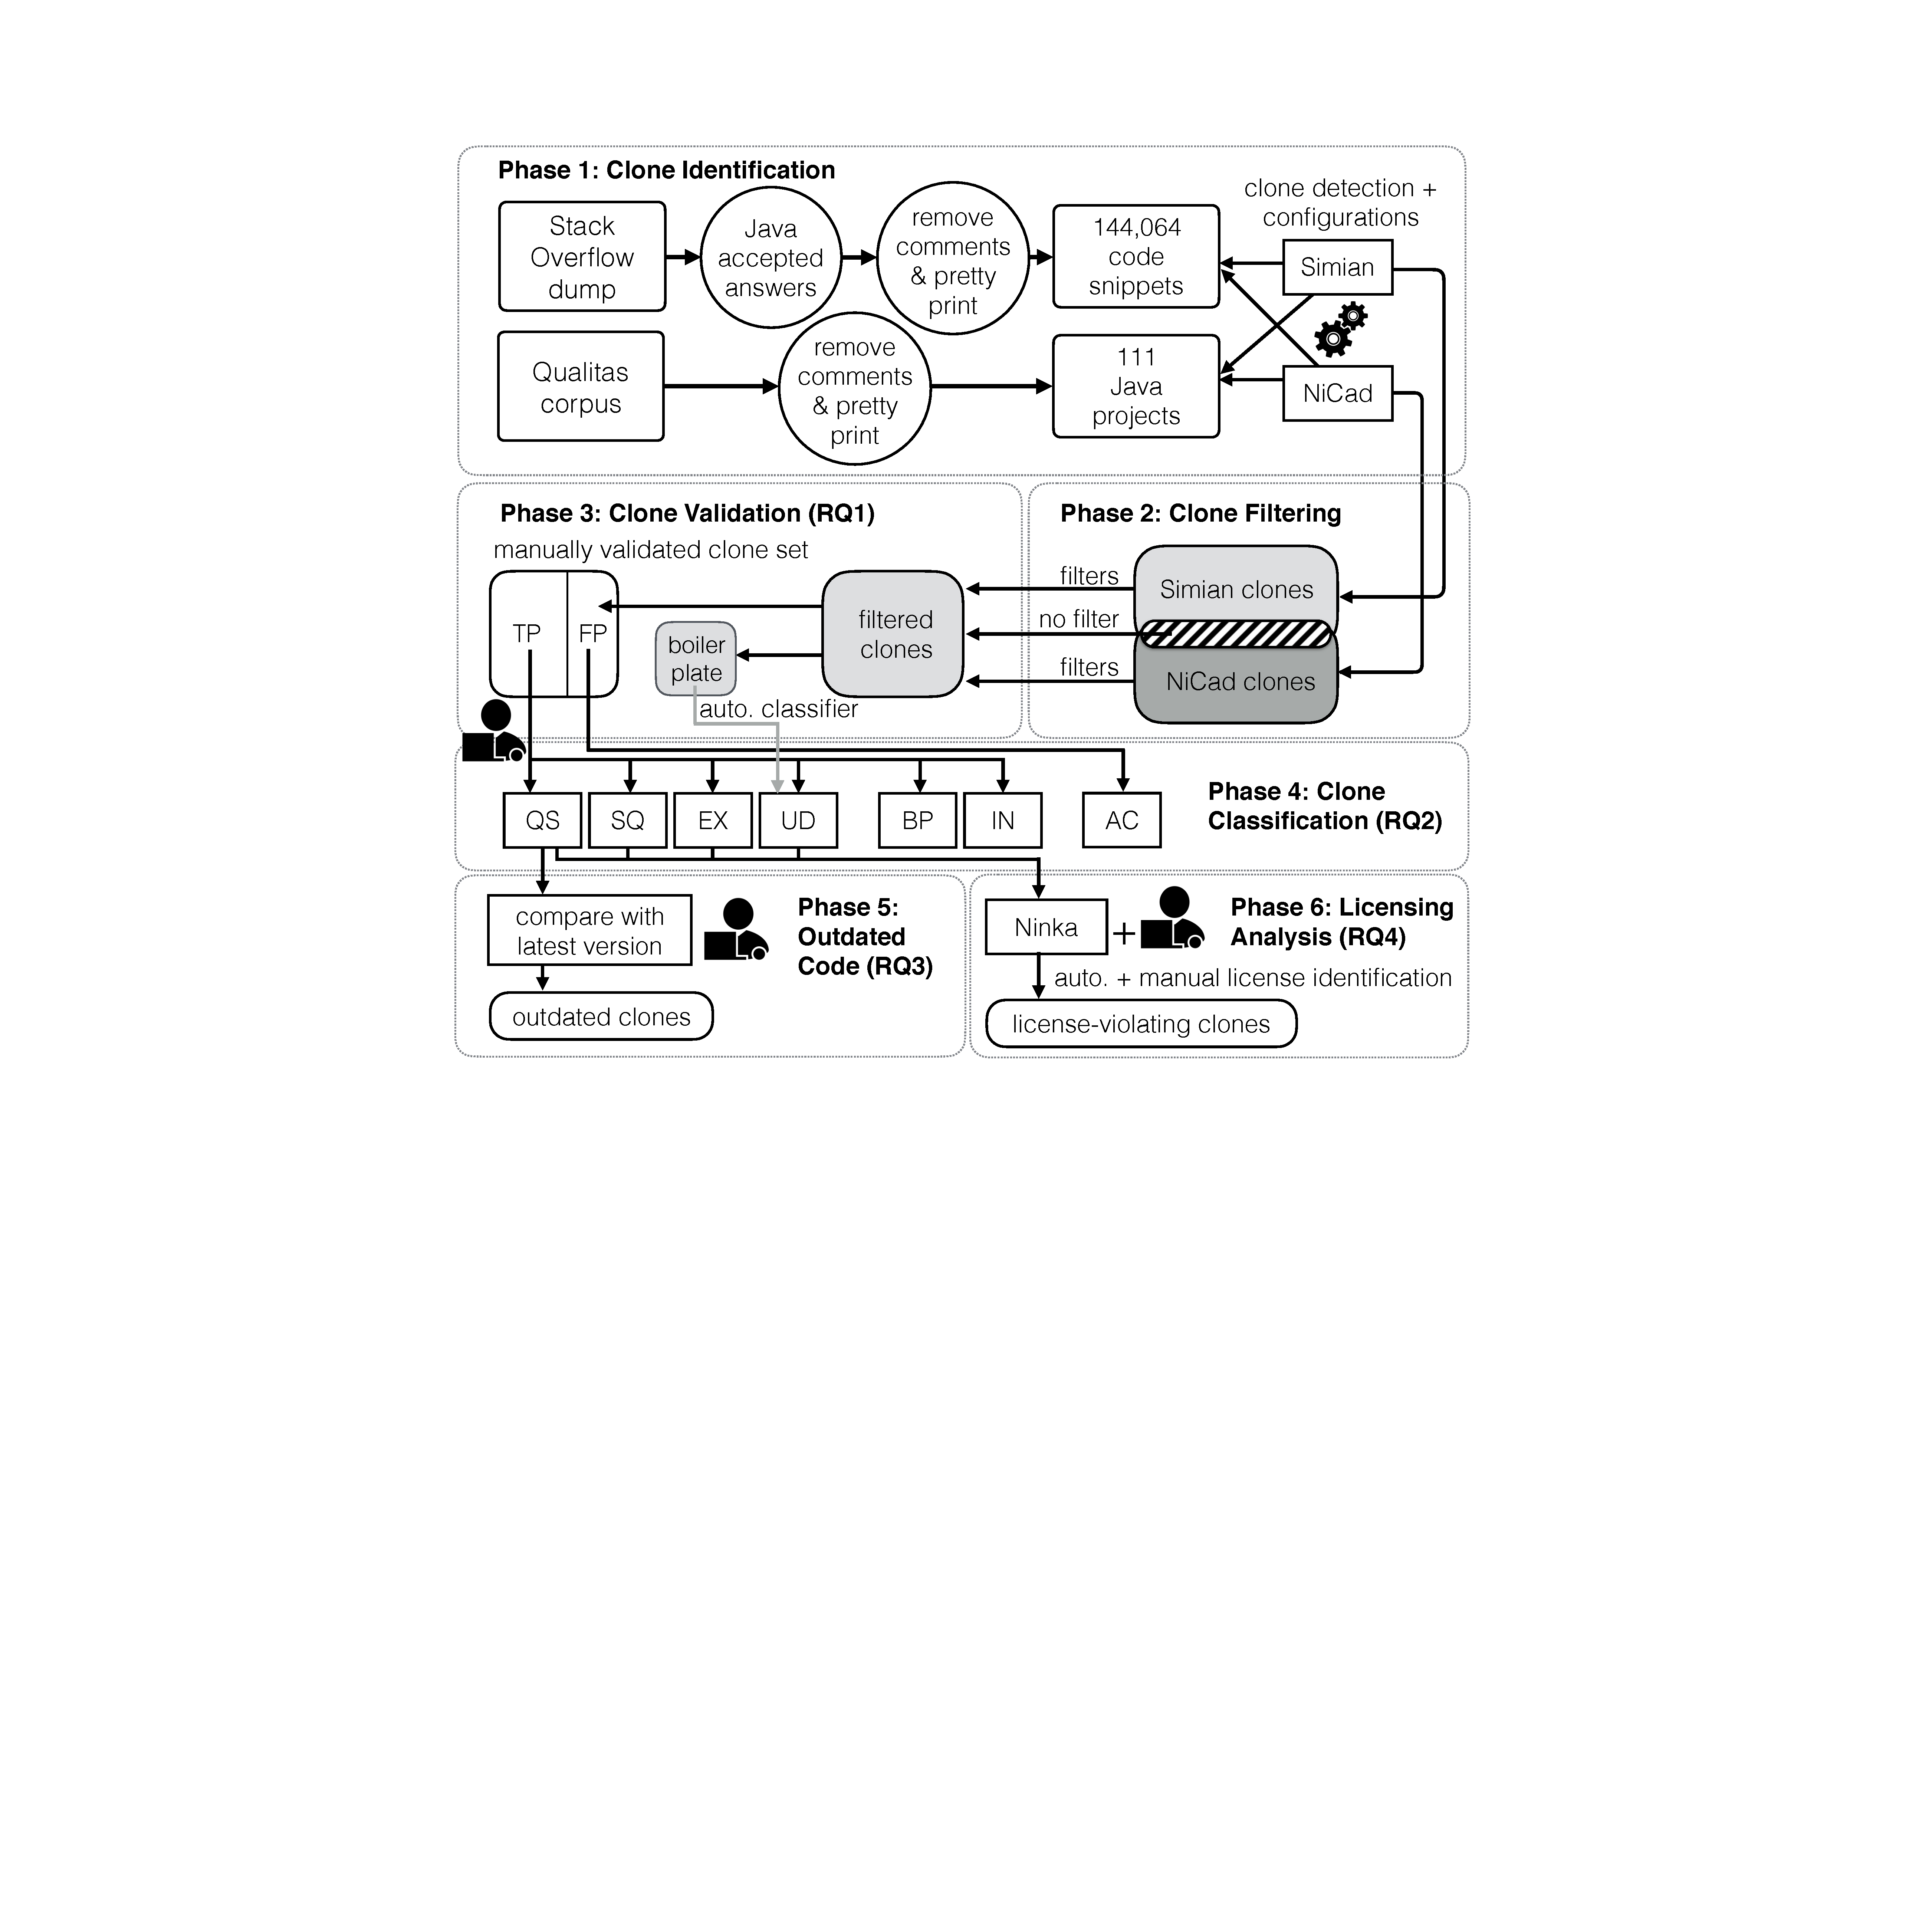
\includegraphics[width=\linewidth]{exp_framework_new}
	\caption{The Experimental framework}
	\label{fig:exp_framework}
\end{figure}

%\subsection{Experimental Setup}
%\vspace{1ex}
To answer these five research questions, we perform two surveys and an empirical study to
understand the developers' awareness of toxic code snippets on Stack Overflow and to
empirically study the online code clones between Stack Overflow and open source
projects, and their toxicity. 

\subsection{Stack Overflow Developers' Survey} We support our motivation of
toxic code snippets on Stack Overflow and answer RQ1 by asking Stack
Overflow users to take an online survey. The survey was used for assessing awareness of
the developers on the two issues of outdated code and license-violating code
snippets. We designed the survey using Google Forms by following the guidelines by Pfleeger and
Kitchenham~\cite{Pfleeger2001,Kitchenham2002}. The survey was completely
anonymous, and the participants could decide to leave at any time. 
We created two versions of the survey: \textbf{the answerer survey} and \textbf{the visitor survey}.
The answerer survey targeted the developers who were experienced Stack Overflow users
and were highly active in answering questions. The visitor survey
targeted the developers who searched for solutions and reused code from Stack Overflow answers.

\textbf{The answerer survey:} the survey contained
11 questions. There were 7 Likert's scale questions, 3 yes/no questions, and one
open-ended question for additional comments. The first two questions were
mandatory while the other 9 questions were shown to the participants based on
their previous answers. The full survey can be found in our research note~\cite{Ragkhitwetsagul_RN2017}.
We selected the participants for the answerer survey based on their Stack Overflow
reputation. On Stack Overflow, a user's reputation reflects how much the
community trusts them. A user earns reputations when he or she receives upvotes
for good questions and useful answers. Accepted answers receive more reputation
score than questions and regular answers\footnote{Stack Overflow
	Reputation:~\url{https://stackoverflow.com/help/whats-reputation}}. Thus, Stack
Overflow reputation is an indicator of user's skills and their involvement in
asking and answering questions on the site. In this study, we call Stack
Overflow users who have a high reputation ``Stack Overflow answerers.''
The participants were invited to take the survey via email addresses available
on their public Stack Overflow and GitHub profiles. We selected the answerers
based on the all-time reputation ranking\footnote{Stack Overflow Users (data as
	of 25 July 2017):~\url{https://stackoverflow.com/users?tab=Reputation&filter=all}}. The
invited participants had a reputation from 963,731 (the highest) to 6,999, and
we sent out 607 emails (excluding undelivered ones, e.g.,\ due to
illegal email addresses). 
The survey was
open for participation for two months, from 25 July to 25 September 2017, before
we collected and analysed the responses.

\textbf{The visitors' survey}
The survey consists of 16 questions: 9 Likert's
scale questions, 3 yes/no questions, 2 multiple-choice questions, and 2
open-ended questions. 
The first four questions are mandatory while the other 12
questions will be shown to the participants based on their previous answers. 
The survey collects information about the participant's software development
experience, the importance of Stack Overflow, reasons for reusing Stack Overflow
snippets, problems from Stack Overflow snippets, licensing of code on Stack
Overflow, and additional feedback. 
The full survey can be found in our research note~\cite{Ragkhitwetsagul_RN2017}.
We adopted non-probability convenient sampling to invite participants for this
survey. Participation in the survey requires experience of visiting Stack
Overflow for solving programming tasks at least once. The participants were
invited to take the survey via five channels: social media post (Facebook),
\textsf{blognone.com} (a popular technology news and media community in Thailand), 
the University of Molise in Italy where the third author
works, the \texttt{comp.lang.java.programmer} group, and the Software Engineering
Facebook page. 
The survey was open for participation for 2 months 
from 25 July 2017 to 25 September 2017.

\subsection{Empirical Study of Online Code Clones}
We support the motivation and confirm the findings in the surveys by performing
an empirical study of online code clones between Stack Overflow
answers and 111 Java open source projects.
We designed the study in 6 phases as depicted in \Cref{fig:exp_framework} where
we build different data sets to answer RQ2 to RQ5. 

\subsubsection{Phase 1: Clone Identification}

We rely on two source code data sets in this study: Java code snippets in answers
on Stack Overflow and open source projects from the Qualitas corpus
\cite{QualitasCorpus}, as detailed next.

\textbf{Stack Overflow:} We extracted Java code snippets from a snapshot of a
Stack Overflow dump\footnote{\url{https://archive.org/details/stackexchange}} in
January 2016. % The archived dump has a size of 9 gigabytes.
The data dump is in XML, and it contains information about posts (questions and
answers). We were interested in code snippets embedded in posts which were
located between {\small\texttt{<code>}...\texttt{</code>}} tags. A Stack
Overflow thread contains a question and several answers. An answer can also be
marked as an \textbf{accepted answer} by the questioner if the solution fixes
his/her problem. We collected Java code snippets using two criteria. First, we
only focused on code snippets in accepted answers. We chose the snippets in
accepted answers because they actually solved the problems in the questions.
Moreover, they are usually displayed just below the questions which makes them
more likely to be reused than other answers. Second, we were only interested in
code snippets of at least ten lines. Although the minimum clone size of six
lines is usual in clone detection~\cite{Bellon2007,Wang2013,Koschke2006}, we
empirically found that snippets of six lines contain a large number of
boiler-plate code of getters/setters, \texttt{equal} or \texttt{hashCode}
methods, which are not interesting for the study. Each snippet was extracted
from the dump and saved to a file. Moreover, we filtered out irrelevant code
snippets that were part of the accepted answers but were not written in Java by
using regular expressions and manual checking.
Finally, we obtained 72,365 Java code snippets containing 1,840,581
lines\footnote{Measured by cloc: \url{https://github.com/AlDanial/cloc}} of Java
source code. The median size of the snippets is 17 lines.

\textbf{Open source systems: }
We selected the established \textbf{Qualitas} corpus~\cite{QualitasCorpus}. It is a curated Java corpus that has been used in several
software engineering
studies~\cite{Taube-Schock2011,Beckman2011,Vasilescu2011,Omar2012}. The
projects in the corpus represent various domains of software systems
ranging from programming languages to
visualisation. We selected the release 20130901r
of the Qualitas corpus containing 112 Java open source projects. This
release contains projects with releases no later than 1st September
2013. We intentionally chose an old corpus from 2013 since we are interested in
online code clones in the direction from open source projects to Stack
Overflow. The 20130901r snapshot provides Java code that is more than
2 years older than the Stack Overflow snapshot, which is sufficiently
long for a number of code snippets to be copied onto Stack Overflow
and also to observe if clones become outdated. Out of 112 Qualitas
projects, there is one project, \textsf{jre}, that does not contain
Java source code due to its licensing limitation~\cite{QualitasCorpus}
and is removed from the study. This resulted in 111
projects analysed in the study, for a total of 166,709 Java files containing 19,614,083
lines of code (see \Cref{tab:datasets}). The median project size is 60,667 lines of code.

\begin{table}
	\centering
	\caption{Stack Overflow and Qualitas datasets}
	\label{tab:datasets}
	%\small
	\begin{tabular}{lrr}
		\toprule
		Data set & No. of files & SLOC \\
		\midrule
		Stack Overflow & 72,365 & 1,840,581 \\ 
		Qualitas &  166,709 & 19,614,083 \\ 
		\bottomrule
	\end{tabular} 
\end{table}

\textbf{Clone Detection Tools: } We use clone detection to discover online code
clones. %\textbf{Clone Detection and Configuration: }
There are a number of restrictions in terms of choosing the clone detection
tools for this study. The main restriction is due to the nature of code snippets
posted on Stack Overflow, as most of them are incomplete Java classes or
methods. Hence, a detector must be flexible enough to process code snippets that
are not compilable or not complete blocks. Moreover, since the amount of code
that has to be processed is in a scale of millions line of code (as shown in
\Cref{tab:datasets}), a clone detector must be scalable enough to report clones
in a reasonable amount of time. We have tried 7 state-of-the-art clone detectors
including Simian~\cite{simian}, SourcererCC~\cite{Sajnani2016},
NiCad~\cite{Cordy,Roy2008}, CCFinder~\cite{Kamiya2002}, iClones~\cite{Gode2009},
DECKARD~\cite{Jiang2007a}, and PMD-CPD~\cite{pmd-cpd} against the Stack Overflow
and Qualitas datasets. NiCad failed to parse 44,960 Stack Overflow snippets
while PMD CPD failed to complete the execution due to lexical errors. iClones
could complete its execution but skipped 367 snippets due to malformed blocks in
Stack Overflow data sets. CCFinder reported 8 errors while processing the two data sets. 
Although Simian, SourcererCC, and DECKARD
could successfully report clones, we decided to choose only Simian and
SourcererCC due to their fast detection speed. Moreover, Simian and
SourcererCC complement each other as SourcererCC's clone fragments are
always confined to method boundaries while Simian's fragments are not.

\textbf{Simian} is a text-based clone detector that locates clones at line-level
granularity and has been used extensively in several clone
studies~\cite{Ragkhitwetsagul2016, emse, Wang2013, Mondal2011, Cheung2015,
  krinke11cloned, Krinke2010, krinke10distinguishing, Krinke2008,
  krinke07study, ragkhitwetsagul18picture}. Furthermore, it offers normalisation of variable names and literals
(strings and numbers) which enables Simian to detect literal clones (type-1) and
parameterised clones (type-2)~\cite{Bellon2007}. \textbf{SourcererCC} is a token-based clone
detector which detects clones at either function- or block-level granularity. It
can detect clones of type-1, -2 up to type-3 (clones with added and removed
statements) and offer scalability against large code
corpus~\cite{Sajnani2016,Saini2016,Yang2017}. 

We prepared the Java code in both datasets by removing comments and
pretty-printing to increase the clone detection accuracy. Then, we deployed the
two detectors to locate clones between the two datasets.  For each Qualitas
project, we ran the tools on the project's code and the entire Stack Overflow
data. Due to incomplete code blocks and functions
typically found in Stack Overflow snippets, the built-in SourcererCC's Java
tokeniser could not parse 45,903 snippets, more than half of them. Nevertheless,
the tool provides an option to plug in a customised tokeniser, so we developed a
special Java tokeniser with assistance from the tool's creators. The customised
tokeniser successfully processed all Stack Overflow snippets.

Simian did not provide an option to detect cross-project clones. Hence the
Simian clone report was filtered to contain only clone pairs between Stack
Overflow and Qualitas projects, removing all clone pairs within either Stack
Overflow or Qualitas. 
SourcererCC can detect cross-project clones between two systems, so we did
not filter the clones.

\begin{table}
	\centering
	\caption{Configurations of Simian and SourcererCC}
	\label{tab:clone_config}
	\begin{tabular}{lp{5cm}}
		\toprule
		Tool & Configurations \\
		\midrule
		Simian~(\textit{S}) &  Threshold=10, ignoreStringCase, \newline ignoreCharacterCase, \newline ignoreModifiers \\ 
		\midrule
		SourcererCC~(\textit{SCC}) & Functions, Minimum clone size=10, \newline Similarity=80\% \\
		\bottomrule
	\end{tabular}
\end{table}

\textbf{Clone Detection Configuration: } We are aware of effects of
configurations to clone detection results and the importance of searching for
optimised configurations in empirical clone
studies~\cite{Svajlenko2014,Wang2014,cr2016ssbse,Ragkhitwetsagul2016, emse}. However,
considering the massive size of the two datasets and the search space of at
least 15 Simian and 3 SourcererCC parameters, we are unable to search for the
best configurations of the tools. Thus, we decided to configure Simian and
SourcererCC based on their established default configurations chosen by the
tools' creators as depicted in \Cref{tab:clone_config}. 
The two clone detectors complemented each
other by having Simian detecting literal copies of code snippets (type-1) and SourcererCC
detecting clones with renaming and added/deleted statements (type-2, type-3). 

Nevertheless, we investigated a crucial parameter setting for clone detection: 
the minimum clone size threshold.
Choosing a large threshold value can reduce the number of trivial clones
(e.g.,~\texttt{equals}, \texttt{hashCode}, or getter and setter methods) and
false clones in the analysis or the manual investigation
phase~\cite{Sajnani2016}, i.e.,~increasing precision. 
Nonetheless, it may create some false negatives. 
On the other hand, setting a low threshold
results in a larger number of clone candidate pairs to look at, i.e.,~increasing recall, 
and a higher chance of getting false positives. 
%It is known that lowering the threshold value 
%is harmful to precision. 
Moreover, the large number of clone
pairs hinders a full manual validation of the clones.
% and one needs to
%rely on sampling of clone pairs. 
Three threshold values, six, ten, and fifteen lines, were chosen for our
investigation. We started our investigation by using a threshold value of six
lines, a well-accepted minimum clone size in clone benchmark~\cite{Bellon2007}.
Simian reported 67,172 clone candidate pairs and SourcererCC reported 7,752
clone candidate pairs. We randomly sampled 382 pairs from the two sets for
a manual check. This sample number was a statistically significant sample with a
95\% confidence level and $\pm 5\%$ confidence interval. The first author
investigated the sampled clone pairs and classified them into three groups:
not clones, trivial clones (\texttt{equals}, \texttt{hashCode}, or getter and
setter methods), and non-trivial clones. The manual check found 26 non-clone
pairs, 322 trivial clone pairs, and 34 non-trivial clone pairs. Next, we increased the
threshold to ten lines, another well-established minimum clone size for
large-scale data sets~\cite{Sajnani2016}, and retrieved 721 clone pairs from
Simian and 1,678 clone pairs from SourcererCC. We randomly sampled and manually
checked the same amount of 382 pairs and found 27 non-clone pairs, 253 trivial
clone pairs, and 102 non-trivial clone pairs. Then, we increased the threshold
further to fifteen lines and retrieved 196 clone pairs from Simian and 1,230
clone pairs from SourcererCC. The manual check of the 382 randomly sampled pairs
revealed zero non-clone pairs, 298 trivial clone pairs, and 83 non-trivial clone
pairs.

The findings from the three threshold values show that selecting the minimum clone size 
of ten lines was preferred over six and fifteen lines. First, it generated 
a fewer number of clone pairs than using six lines, which made the manual clone
investigation feasible. Second, it preserved the highest number of non-trivial clone
pairs.
%
%The minimum clone size of 10 lines is
%considered a standard setting for clone detection in large-scale data sets to
%avoid trivial clones (e.g.,~\texttt{equals}, \texttt{hashCode}, or getter and
%setter methods) in the analysis or the manual investigation phase~\cite{Sajnani2016}.  
%We
% performed an analysis to confirm this.
%\begin{figure} 
%	\centering
%	\includegraphics[width=\linewidth]{boxplot_clone_size_combined} 
%	\caption{Size of online code clones.} 
%	\label{fig:boxplotclonesize}
%\end{figure}
%
%The result is as shown in
%\Cref{fig:boxplotclonesize}. We found that the distribution of the manually
%confirmed true clones 
%mainly cover the size from about 10 to 20 lines. Increasing
%the threshold to be higher than 10 would remove some of the
%true clone pairs.
%
%Regarding decreasing the minimum clone size to be less than 10 lines, we reran
%the two clone detection tools again using a minimum
%clone size of 6 lines, another well-accepted minimum clone size in clone
%benchmark~\cite{Bellon2007}. Simian reported 67,172 clone candidate pairs and
%SourcererCC reported 7,752 clone candidate pairs with 776 common clone pairs. 
%With this large amount of clone
%candidate pairs, it is not feasible to manually confirm all of the clones and we
%must rely on sampling. This will result in weaker findings and
%weaker conclusion. Thus, we decide pick the minimum clone size of 10 lines
%to keep the balance between the number of non-trivial clone pairs and the
%feasibility of manual clone investigation.
%We made sure that they 
%detected only non-trivial clones by increasing the minimum clone size to ten
%lines.
%(denoted as \textit{D}), and (2)~the discovered configurations for
%Bellon's Java projects from \textit{EvaClone}~\cite{Wang2013}, a study
%of optimising clone detectors' configurations based on clone agreement
%(denoted by \textit{E}). \Cref{t:param_tuning} shows the two configurations.
%In total, we have four configurations: Simian with the default
%configuration ($S_D$), Simian with the EvaClone configuration ($S_E$), 
%NiCad with the default configuration ($N_D$)
%and NiCad with the EvaClone configuration ($N_E$).
%
%We encountered NiCad failures with a few Qualitas projects.~$N_D$
%could not detect clones in \textsf{hibernate} due to clustering
%errors. $N_E$ generated errors during code normalisation for 5
%projects including \textsf{vuze}, \textsf{hibernate},
%\textsf{myfaces}, \textsf{netbeans}, and \textsf{spring}. We have
%contacted the creator of NiCad regarding the issues. They identified
%the issues as problems in the TXL grammar and as problems of long file
%paths, and will be fixed in the next NiCad releases.
%
The number of online clone pairs reported using the minimum clone size of 10 lines
are presented in \Cref{tab:orig_stats}. Simian reports 721 clone
pairs while SourcererCC reports 1,678 clone pairs. 
%SourcererCC reports more clones due to its capability of detecting
%clones of type-1 to type-3 while Simian only detects type-1 clones.
The average clone size reported by Simian is
16.61 lines which is slightly smaller than SourcererCC (17.86 lines).

\begin{table}
	\centering
	\caption{Number of online clones reported by Simian and SourcererCC}
	\label{tab:orig_stats}
	%\small
	%\resizebox{\columnwidth}{!}{%
	\begin{tabular}{lrr}
		\toprule
		Tool & \multicolumn{1}{c}{Total clone pairs} & \multicolumn{1}{c}{Average clone size} \\
		\midrule
		Simian & 721 & 16.61 \\
		SourcererCC & 1,678 & 17.86 \\
		\bottomrule
	\end{tabular} %
	%}
\end{table}

\subsubsection{Phase 2: Clone Merging} Clones from the two detectors can be
duplicated. To avoid double-counting of the same clone pair, we adopted the idea
of \textbf{clone agreement} which has been used in clone research
studies~\cite{Funaro2010, Wang2013,cr2016ssbse} to merge clones from two data
sets. Clone pairs agreed by both clone detection tools have a high
likelihood to be duplicate and must be merged. 
%By using this agreement-based
%approach, we reduced the number of clone candidates for manual investigation and
%avoid a threat to internal validity of double counting the same clone pair twice
%by merging the ones agreed by the two tools. 
To find agreement between two clone
pairs reported by two different tools, we used the clone pair matching metric
proposed by Bellon et al.~\cite{Bellon2007}. Two clone pairs that have a large
enough number of overlapping lines can be categorised as either a good-match or
an ok-match pair with a
confidence value between 0 and 1. Although good-match has a stronger agreement
than ok-match, we choose the ok-match criterion as our clone merging method
because it depends on clone containment and does
not take clone size into account. Clone containment suits our online code clones
from two tools, Simian (line-level) and SourcererCC (method-level), better
because Simian's clone fragments can be smaller or bigger than a method
while SourcererCC's clone fragments are always confined to a method boundary.

We follow Bellon's original definitions of ok-match~\cite{Bellon2007}, which are based on how much two clone
fragments \textit{CF} are contained in each other:
%\squeezeup
%\begin{displaymath}
%overlap(\textrm{\textit{CF}}_1, \textrm{\textit{CF}}_2) = \frac{|lines(\textrm{\textit{CF}}_1) \cap lines(\textrm{\textit{CF}}_2)|}{|lines(\textrm{\textit{CF}}_1) \cup lines(\textrm{\textit{CF}}_2)|} 
%\end{displaymath}
% \squeezeup
\begin{displaymath}
contained(\textrm{\textit{CF}}_1, \textrm{\textit{CF}}_2) = \frac{|lines(\textrm{\textit{CF}}_1) \cap lines(\textrm{\textit{CF}}_2)|}{|lines(\textrm{\textit{CF}}_1)|}
\end{displaymath}
\noindent%
A clone pair \textit{CP} is formed by two clone fragments
\textit{CF$_1$} and \textit{CF$_2$}, i.e.,~\textit{CP} =
(\textit{CF$_1$}, \textit{CF$_2$})
%, and the \textit{good-value} and
and the \textit{ok-value} of two clone pairs is defined as
%\squeezeup
%\begin{align*}
%good(\textrm{\textit{CP}}_1, \textrm{\textit{CP}}_2) = min(overlap(\textrm{\textit{CP}}_1.\textrm{\textit{CF}}_1,\textrm{\textit{CP}}_2.\textrm{\textit{CF}}_1), \\ overlap(\textrm{\textit{CP}}_1.\textrm{\textit{CF}}_2,\textrm{\textit{CP}}_2.\textrm{\textit{CF}}_2))
%\end{align*}
\begin{align*}
ok(\textrm{\textit{CP}}_1,\textrm{\textit{CP}}_2) = min(max(contained(\textrm{\textit{CP}}_1.\textrm{\textit{CF}}_1,\textrm{\textit{CP}}_2.\textrm{\textit{CF}}_1),~~ \\ contained(\textrm{\textit{CP}}_2.\textrm{\textit{CF}}_1,\textrm{\textit{CP}}_1.\textrm{\textit{CF}}_1)),~
\\ max(contained(\textrm{\textit{CP}}_1.\textrm{\textit{CF}}_2,\textrm{\textit{CP}}_2.\textrm{\textit{CF}}_2),~~ \\contained(\textrm{\textit{CP}}_2.\textrm{\textit{CF}}_2,\textrm{\textit{CP}}_1.\textrm{\textit{CF}}_2)))
\end{align*}

\noindent%
Two clone pairs $\textrm{\textit{CP}}_1$ and $\textrm{\textit{CP}}_2$
are called an \textit{ok-match(t)}  iff, for threshold $t \in [0,1]$ holds 
%\squeezeup
\begin{align*}
%good(\textrm{\textit{CP}}_1,\textrm{\textit{CP}}_2) & \geq t\\
ok(\textrm{\textit{CP}}_1,\textrm{\textit{CP}}_2) & \geq t
\end{align*}

The threshold \textit{t} is crucial for the ok-match because it affects the number
of merged clone pairs. Setting a high \textit{t} value will result in a few ok-match clone pairs
and duplicates of the same clone pairs (which are supposed to be merged) may appear in the merged
clone set. On the other hand, setting a low \textit{t} value will result in many ok-match clone
pairs, and some non-duplicate clone pairs may be accidentally merged by only
a few matching lines.
In order to get an optimal $t$ value, we did an analysis by choosing
five $t$ values of 0.1, 0.3, 0.5, 0.7, 0.9 and studied the merged clone candidates.
By setting $t=0.7$ according to Bellon's study, we
found 97 ok-match pairs reported. On the other hand, setting $t$ to 0.1, 0.3,
0.5, and 0.9 resulted in 111, 110, 110, and 94 ok-matched pairs respectively.
Since the clone pairs of $t=0.1$ were the superset of other sets,  we manually
checked all the 111 reported pairs. We found one false positive pair and 110
true positive pairs. By raising the $t$ to 0.3 and 0.5, we got rid of the false
positive pair and still retained all the 110 true positive pairs. All the clone
pairs of $t=0.7$ (97) and $t=0.9$ (94) were also true positives due to being a
subset of $t=0.5$. However, since there were fewer merged clone pairs, 
we ended up leaving some duplicates of the same clones in the final merged clone set.
With this analysis, we can see that setting the threshold $t$ to 0.1 is too
relaxed and results in having false positive ok-match pairs, while setting the
$t$ to 0.7 or 0.9 is too strict. Thus,
we decided to select the $t$ value at 0.5. 

Using the ok-match criterion with the threshold \textit{t} of 0.5
similar to Bellon's study~\cite{Bellon2007}, we merge 721 clone pairs from
Simian and 1,678 clone pairs from SourcererCC into a single set of 2,289 online
clone pairs. There are 110 common clone pairs between the two clone sets 
as depicted in~\Cref{fig:clonemerging}.  The low number of common
clone pairs is due to SourcererCC reporting clones with method
boundaries while Simian is purely line-based.

\begin{figure}
	\centering
	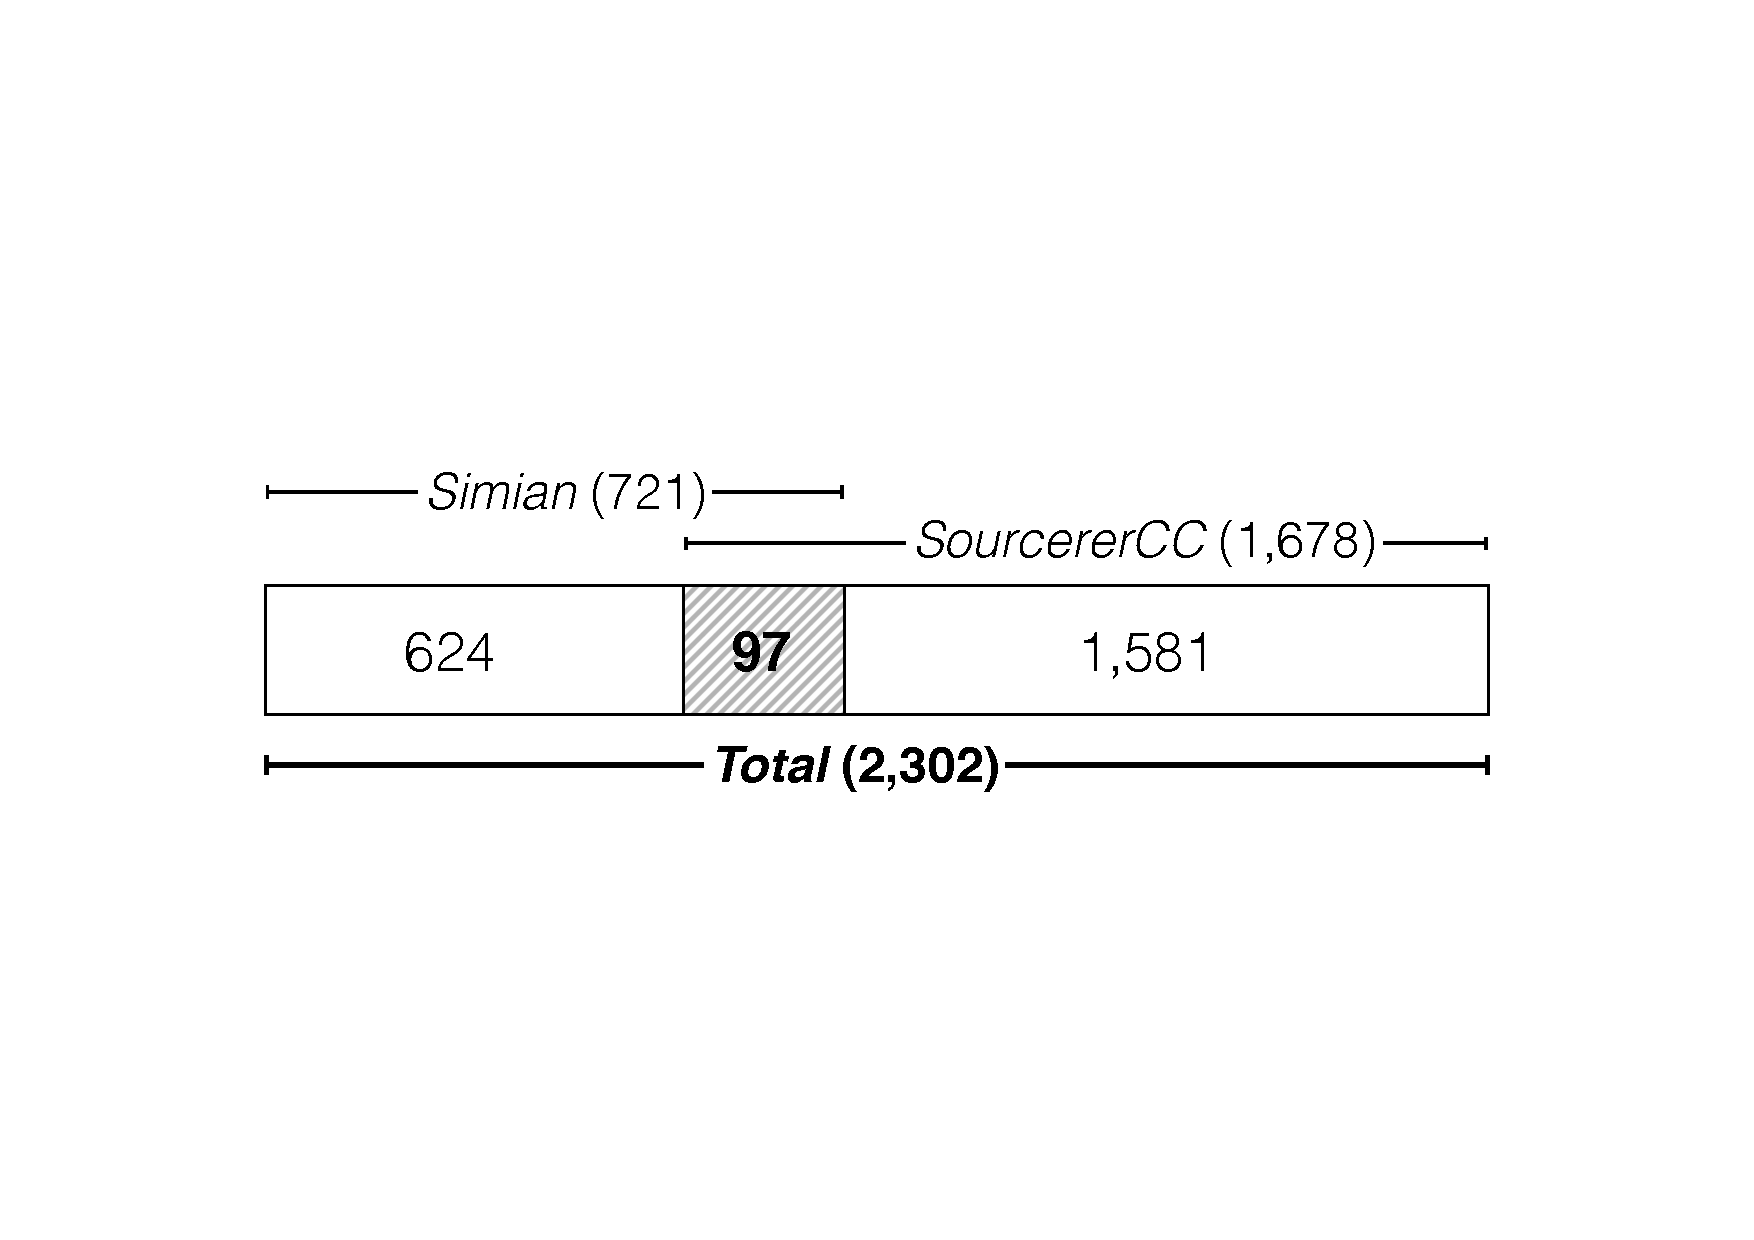
\includegraphics[width=0.8\linewidth]{clone_merging}
	\caption{The result from clone merging using Bellon's ok-match criterion}
	\label{fig:clonemerging}
\end{figure}

\subsubsection{Phase 3-4: Validation and Classification}
We used the 2,289 merged clone pairs for
manual validation and online clone classification.
The validation and classification of the pairs were done at the same time. 
The clone validation process (phase 3 in \Cref{fig:exp_framework}) involves checking 
if a clone pair is a true positive or a false positive. 
Moreover, we are also interested in 
the patterns of code cloning so we can gain more insights into 
how these clones are created (phase 4 in \Cref{fig:exp_framework}). 

\textbf{Manual investigation:} 
To mitigate the human error, we deployed two people in the manual clone
investigation process. The first author, who is a research student working on
clone detection research for three years, and the third author, who is a
software engineering research student and familiar with code clones, took the
role of the investigators performing a manual validation and classification of
the merged clone pairs. The two investigators separately went through each clone
pair candidate, looked at the clones, and decided if they are a true positive or
a false positive and classified them into an appropriate pattern. After the
validation, the results from the two investigators were compared. 
%and 607 (26\%)
%conflicts were discussed and resolved. 
There were 338 (15\%) conflicts between 
true and false clones (QS, SQ, EX, UD, BP, IN vs.~NC).
The investigators looked at each conflicting pair together and
discussed until a consensus was made. 
Another 270 pairs (12\%) were
conflicts in the classification of
the true clone pairs. Among these pairs, 145 conflicts were caused by
one investigator being more careful than the other and being able to find evidence of 
copying while the other could not. Thus, resolving the conflicts lead to a better classification,
 i.e.,~from UD to QS or EX.
%There were three conflicts where the two
%investigators could not find a consensus and the third author was involved for
%the final judgement.

% No. of conflicts = 37 (ok) + 352 (simian) + 218 (SCC)
% 33 pairs are changed from MP.UD --> CR.EX,QS
% 112 pairs are changed from CR.UD --> MP.EX,QS

\begin{table}
	\centering
	\caption{The seven patterns of online code cloning}
	\label{tab:classification_scheme}
	%\resizebox{\columnwidth}{!}{%
	\begin{tabular}{c@{~~}p{7.35cm}}
		\toprule
		Patt. & Description \\ 
		\midrule
		QS & Cloned from Qualitas project to Stack Overflow (Q $\rightarrow$ S) \\ 
		
		SQ & Cloned from Stack Overflow to Qualitas project (S $\rightarrow$ Q) \\ 
		
		EX & Cloned from an external source to Stack Overflow (X $\rightarrow$ S) \\
		
		UD & Cloned from each other or from an external source
                     outside the project (unknown)\\
		\midrule
		BP & Boiler-plate or IDE auto-generated \\ 
		
		IN & Inheritance, interface implementation  \\ 
		
		NC & Not clones \\ 
		\bottomrule 
	\end{tabular}  %
	%}
\end{table}

\textbf{The online cloning classification patterns:} 
We studied the eight patterns of cloning from Kapser et
al.~\cite{Kapser2006,Kapser2008} and performed a preliminary study to
evaluate its applicability to our study. 
We tried to classify 697 online clone pairs from
the reported clones in phase 1 
%Using the $S_D$ clone report,
%snippets were ranked according to (1)~clone pair frequency,
%(2)~popularity (i.e.,~number of associated Qualitas projects),
%(3)~clone size in SLOC, and (4)~ratio of cloned code per snippet. We
%selected these four criteria so that we could cover the online clones
%from various aspects. We selected the top 10 from each ranking and
%obtained 34 unique Stack Overflow snippets. The snippets were
%associated with 697 clone pairs.
%\subsection{Defining Online Code Cloning Patterns}
using Kapser's cloning patterns. We found that 
% the
% clone pairs were categorised into either Customisation or Templating.
% Thus, 
Kapser's patterns are too broad for our study and a more suitable and
fine-grained classification scheme is needed. After a preliminary study, we
adopted one of Kapser's cloning patterns, \emph{boiler-plate code}, and defined
six new cloning patterns. The seven patterns include QS, SQ, EX, UD, BP, IN, and
NC as presented in \Cref{tab:classification_scheme}. Pattern QS
(\textbf{Q}ualitas to \textbf{S}tack Overflow) represents clones that have
evidence of being copied from a Qualitas project to Stack Overflow. The evidence
of copying can be found in comments in the Qualitas source code or in the Stack
Overflow post's contents. Pattern SQ (\textbf{S}tack Overflow to
\textbf{Q}ualitas) is cloning, with evidence, in the opposite direction from
Stack Overflow to a Qualitas project. Pattern EX (\textbf{Ex}ternal Sources) is
cloning that has evidence of copying from a single or multiple external sources
to Stack Overflow, and possibly also to a Qualitas project.  Pattern UD
(\textbf{U}nknown \textbf{D}irection) is cloning that creates identical or
highly similar clones between Qualitas and Stack Overflow but where we could not
find any attribution of copying. Pattern BP (\textbf{B}oiler-\textbf{P}late)
represents clones containing boiler-plate. We define three cases of boiler-plate
code and use in our classification as shown in \Cref{tab:boiler-plate_code}. Our
definition is specific to Java and more suitable to our study than the general
definition in Kapser's~\cite{Kapser2008}.
%of {\small\verb|equals()|} methods,
%getters/setters, well-known code patterns such as deleting a file
%or implementing a {\small{\texttt{toString}} method,
% or IDE-generated code such as GUI components. 
 Pattern
IN (\textbf{In}heritance/Interface) is cloning by inheritance of the
same super class or implementation of the same interface. These two
activities usually result in similar overriding methods. The last
pattern, NC (\textbf{N}ot \textbf{C}lones), represents
false clone pairs. These are mainly false positive
clones from the clone detectors such as similar
{\small\texttt{try-catch}} statements.

\begin{table}
	\centering
	\caption{The definition of boiler-plate code}
	\label{tab:boiler-plate_code}
	\begin{tabular}{lp{5.5cm}}
		\toprule
		Type & Description \\ 
		\midrule
		\textbf{API constraints} & Similar code fragments are created because of a constraint by an API. For example, reading and writing to database using JDBC, reading and writing a file in Java. \\
		\midrule
		\textbf{Templating} & An optimised or stable code fragment is reused multiple times. This also includes auto-generated code by IDE. \\
		\midrule
		\textbf{Design patterns} & Java design patterns suggest a way of implementing similar pieces of code. For example, getters, setters, {\small\texttt{equals}}, {\small\texttt{hashCode}}, and {\small\texttt{toString}} method. \\
		\bottomrule 
	\end{tabular}  %
	%}
\end{table}

\begin{figure}
	\centering
	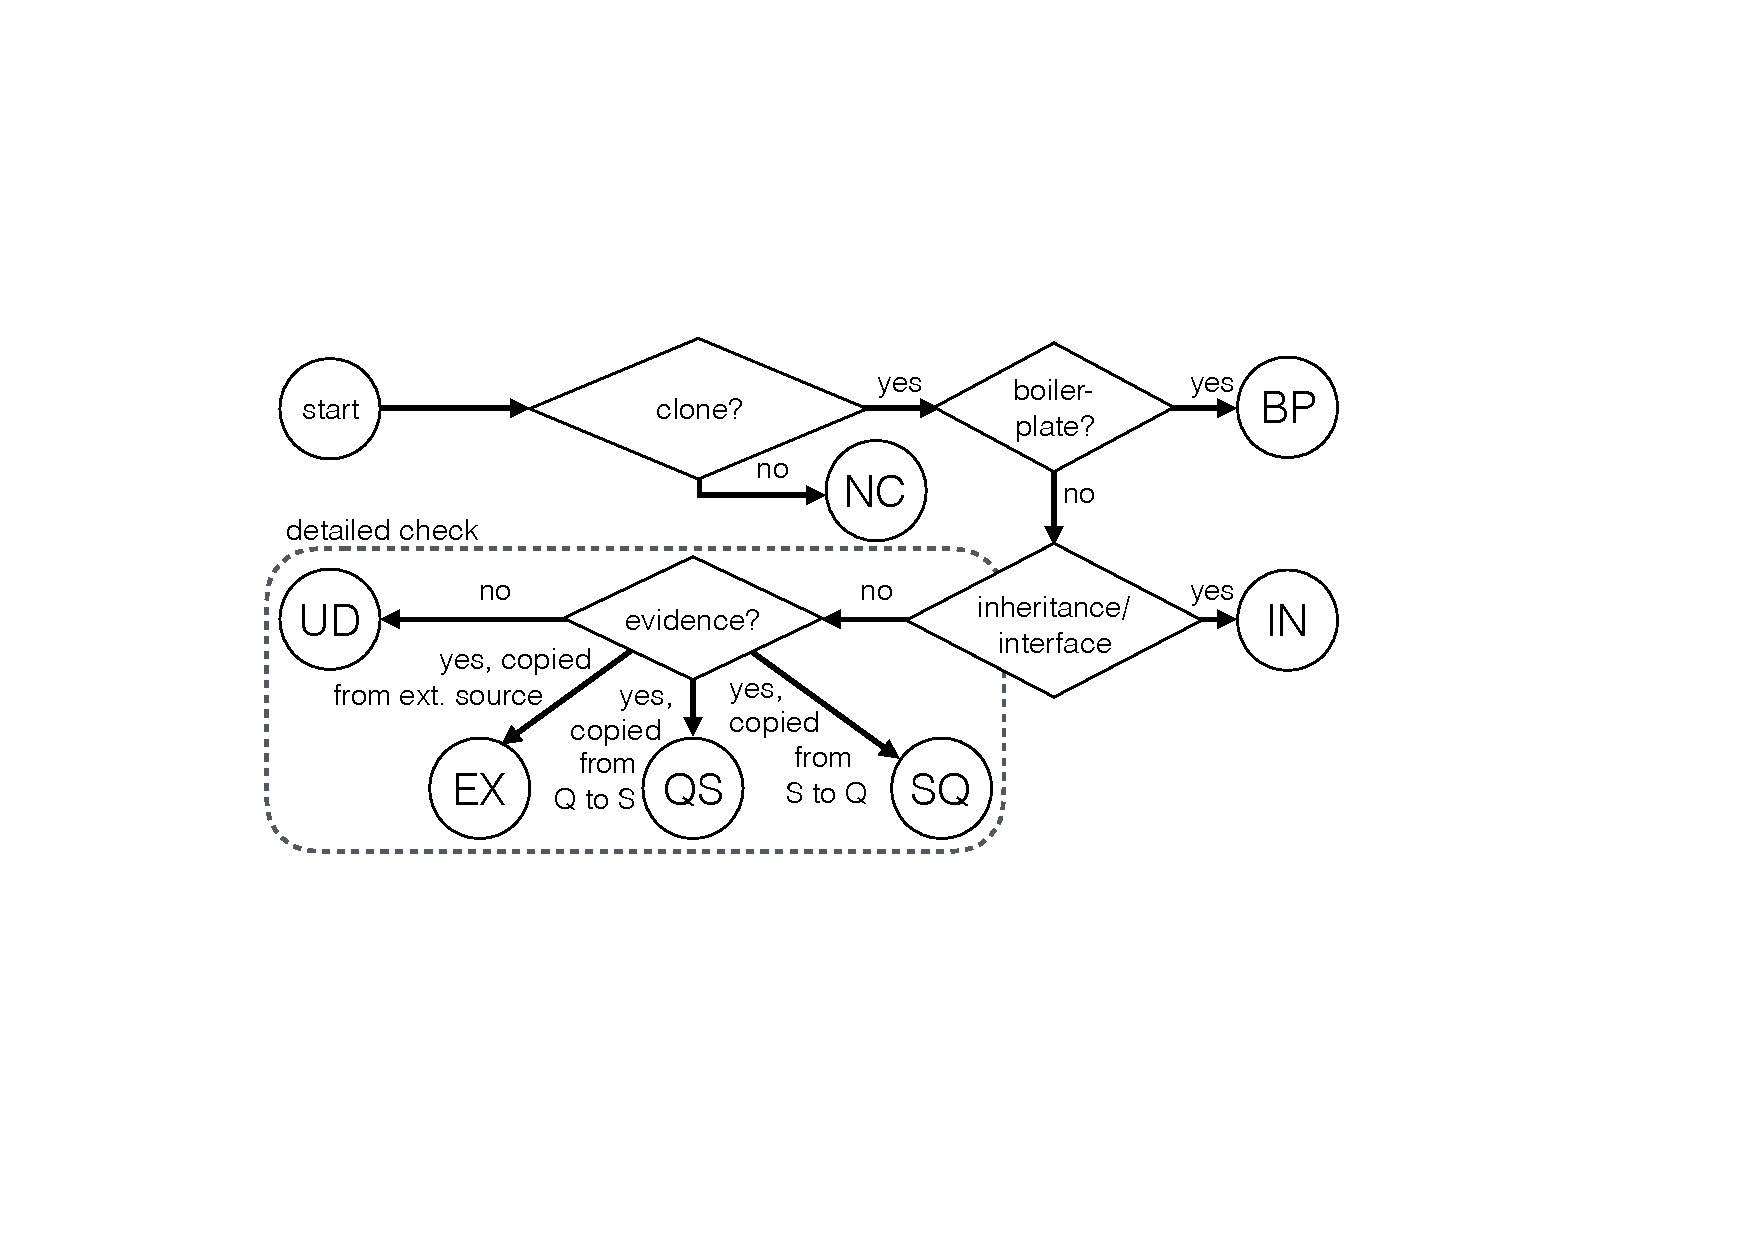
\includegraphics[width=0.9\linewidth]{classification_process}\vspace{-1ex}
	\caption{Online code clone classification process}
	\label{fig:classification_process}
\end{figure}

The classification of the filtered online clone pairs followed the steps
depicted in \Cref{fig:classification_process}. First, we look at a pair of clone
fragments to see their similarity. If they are accidentally similar code fragments after
code normalisation or false positive clones from the clone detection tools, we
classify the pair into \textbf{NC}. If the two fragments are boiler-plate code,
the pair is classified into \textbf{BP}. If they implement the same interface or
inherited the same class and share similar overriding methods, the pair is
classified into \textbf{IN}. If the pair is not \textbf{BP}, \textbf{IN}, or
\textbf{NC}, we start a detailed investigation. We check the corresponding Stack
Overflow post, read through it carefully and look for any evidence mentioning
code copying. If evidence of copying has been found from a Qualitas project, the
pair is classified in \textbf{QS}. In several occasions, we used extra
information such as the questions' contents, the name of posters, and the tags to gain a
better understanding. On the other hand, if the source code from the Qualitas
project mentions copying from Stack Overflow, the pair is classified into
\textbf{SQ}. If there is evidence of copying from an external source instead of
a Qualitas project, the pair is classified as \textbf{EX}. Lastly, if there
is no evidence of copying in any direction but the clone fragments are highly
similar, we classify them into \textbf{UD}.

\subsubsection{Phase 5: Outdated Clones} Outdated code occurs when a piece of code
has been copied from its origin to another location, and later the original has
been updated~\cite{Xia2014}. Usually, code clone detection is used to locate
clone instances and update them to match with the originals~\cite{Bellon2007}.
However, online code clones are more difficult to detect than in regular
software projects due to its large search space and a mix of natural and
programming languages combined in the same post.

To search for outdated online code clones, we focused on the \textbf{QS} clone
pairs that were cloned from Qualitas to Stack Overflow and compared them with
their latest versions. We downloaded the latest version of the Qualitas projects
from their repositories on October 3, 2017. For each \textbf{QS} online clone
pair, we used the clone from Qualitas as a proxy. We searched for its latest
version by the file name and located the cloned region in the file based on the
method name or specific code statements. We then compared the Stack Overflow
snippet to its latest version line-by-line to find if any change has been made
to the source code. We also made sure that the changes did not come from the
modifications made to the Stack Overflow snippets by the posters but from the
updates in the projects themselves. When we found inconsistent lines between the
two versions, we used {\small\texttt{git blame}} to see who modified those lines
of code and the timestamps. We also read commit messages and investigated the issue tracking information
if the code change is linked to an automatic issue tracking system, such as Jira
or BugZilla to gain insights into the intent behind the change.

Lastly, we searched for the outdated code snippets in 130,719 GitHub projects to
see how widespread is the outdated code in the wild. We mined GitHub
based on the number of stars the projects received, which indicated their popularity. We relied on
GitHub API to query the project metadata before cloning them.
Since GitHub API returned only top 1,000 projects at a time for each query, we formulated the
query to retrieve most starred projects based on their sizes.
The project size range started from 1KB to 2MB with 1KB step size, and the last query is
for all the remaining projects that were larger than 2MB.
With this method, we retrieved the top 1,000 most starred projects for each project size. 
As a result, we cloned 130,719 GitHub projects ranging from 29,465 stars to 1 star.
A clone detection was then performed between the outdated code snippets and the GitHub
projects. We selected SourcererCC with the same settings (see \Cref{tab:clone_config}) 
for this task because it could scale to a large-scale data set, while Simian could not. Finally, we analysed
the clone reports and manually checked the clones.

\subsubsection{Phase 6: Licensing Analysis} Software licensing plays an important
role in software development. Violation of software licenses impacts software
delivery and also leads to legal issues~\cite{Sprigman2015}. 
One can run into a licensing issue if one integrates third-party source code
into their software without checking. A study by An et al.~\cite{An2017} reports
1,279 cases of potential license violations between 399 Android apps and Stack
Overflow code snippets.

We analysed licensing conflicts of the online clones in the \textbf{QS},
\textbf{EX}, and \textbf{UD} set. The licenses were extracted by \emph{Ninka},
an automatic license identification tool~\cite{German2010}. Since Ninka works at
a file level, we report the findings based on Stack Overflow snippets and Qualitas
source files instead of the clone pairs (duplicates were ignored). For the ones
that could not be automatically identified by Ninka and have been reported as
{\small\texttt{SeeFile}} or {\small\texttt{Unknown}}, we looked at them manually
to see if any license can be found. For EX clone pairs that are cloned from
external sources such as JDK or websites, we manually searched for the license
of the original code. Lastly, we searched for occurrences of the license-conflicting
online clones in GitHub projects using the same method as in the outdated clones.

\section{Results and Discussion}

We use the two online surveys of Stack Overflow answerers and visitors to answer RQ1
and follow the 6 phases in the experimental framework
(\Cref{fig:exp_framework}) to answer the other four research questions. To answer RQ2,
we rely on the number of manually validated true positive online clone pairs in
phase 3. We use the results of the manual classification by the seven patterns
of online code cloning to answer RQ3 (phase 4). For RQ4, we looked at the true
positive clone pairs that are classified as clones from Qualitas to Stack
Overflow and checked if they have been changed after cloning (phase 5).
Similarly, for RQ5, we looked at the license of each clone in the pattern QS,
EX, UD and checked for a possibility of license violation (phase 6). 

\subsection{RQ1: Stack Overflow Answerers' and Visitors' Awareness}

%\begin{table}
%	\centering
%	\caption{Stack Overflow answerers taken the survey}
%	\label{tab:survey_target}
%	\begin{tabular}{rrrr}
%		\toprule
%		Reputation & Sent emails & Answers & Rate \\
%		\midrule
%		963,731--6,999 & 607 & 201 & 33\% \\
%		\bottomrule
%	\end{tabular}
%\end{table}

\subsubsection{The Answerer Survey}

We received 201 answers (33\% response rate) from 607 emails we sent to the
Stack Overflow answerers. The response rate was high considering other
online surveys in software engineering~\cite{Punter2003}. 
We only present a summary of the survey answers in
this paper, and the full analysis is available as a research note~\cite{Ragkhitwetsagul_RN2017}.

\textbf{General Information:} As shown in \Cref{tab:survey_exp}, the majority of the answerers are experienced
developers with more than 10 years of experience (55.2\%) or between 5 to 10
years (28.9\%). They are active users and regularly answer questions. 49
participants (24\%) answer questions on Stack Overflow every day.

\begin{table}
	\centering
	\caption{Experience of Stack Overflow answerers}
	\label{tab:survey_exp}
	\begin{tabular}{lrr}
		\toprule
		Experience & Amount & Percent \\
		\midrule
		Less than a year & 1 & 0.5\% \\
		1 -- 2 years & 1 & 0.5\% \\
		3 -- 5 years & 30 & 14.9\% \\
		5 -- 10 years & 58 & 28.9\% \\
		More than 10 years	& 111 & 55.2\% \\
		\bottomrule
	\end{tabular}
\end{table}

\begin{table}
	\centering
	\caption{Frequency of including code snippets in answers}
	\label{tab:survey_code_snippet_frequency}
	\begin{tabular}{lrr}
		\toprule
		Include code snippets & Amount & Percent \\
		\midrule
		Very Frequently (81--100\% of the time)	& 84 & 42\% \\
		Frequently (61--80\% of the time) &	63 & 31\% \\
		Occasionally (41--60\% of the time) & 40 & 20\% \\
		Rarely (21--40\% of the time) & 11 & 6\% \\
		Very Rarely (1--20\% of the time) & 2 & 1\% \\
		Never (0\% of the time) & 1 & 1\% \\
		\midrule
		Total & 201 & 100\% \\
		\bottomrule
	\end{tabular}
\end{table}

\textbf{Code Snippets in Answers:}
84 and 63 answerers include code snippets in more than 80\% and 60\% of
their answers respectively. Interestingly, there is one answerer who never
include code snippet in his/her answers (\Cref{tab:survey_code_snippet_frequency}).

\begin{figure}
	\centering
	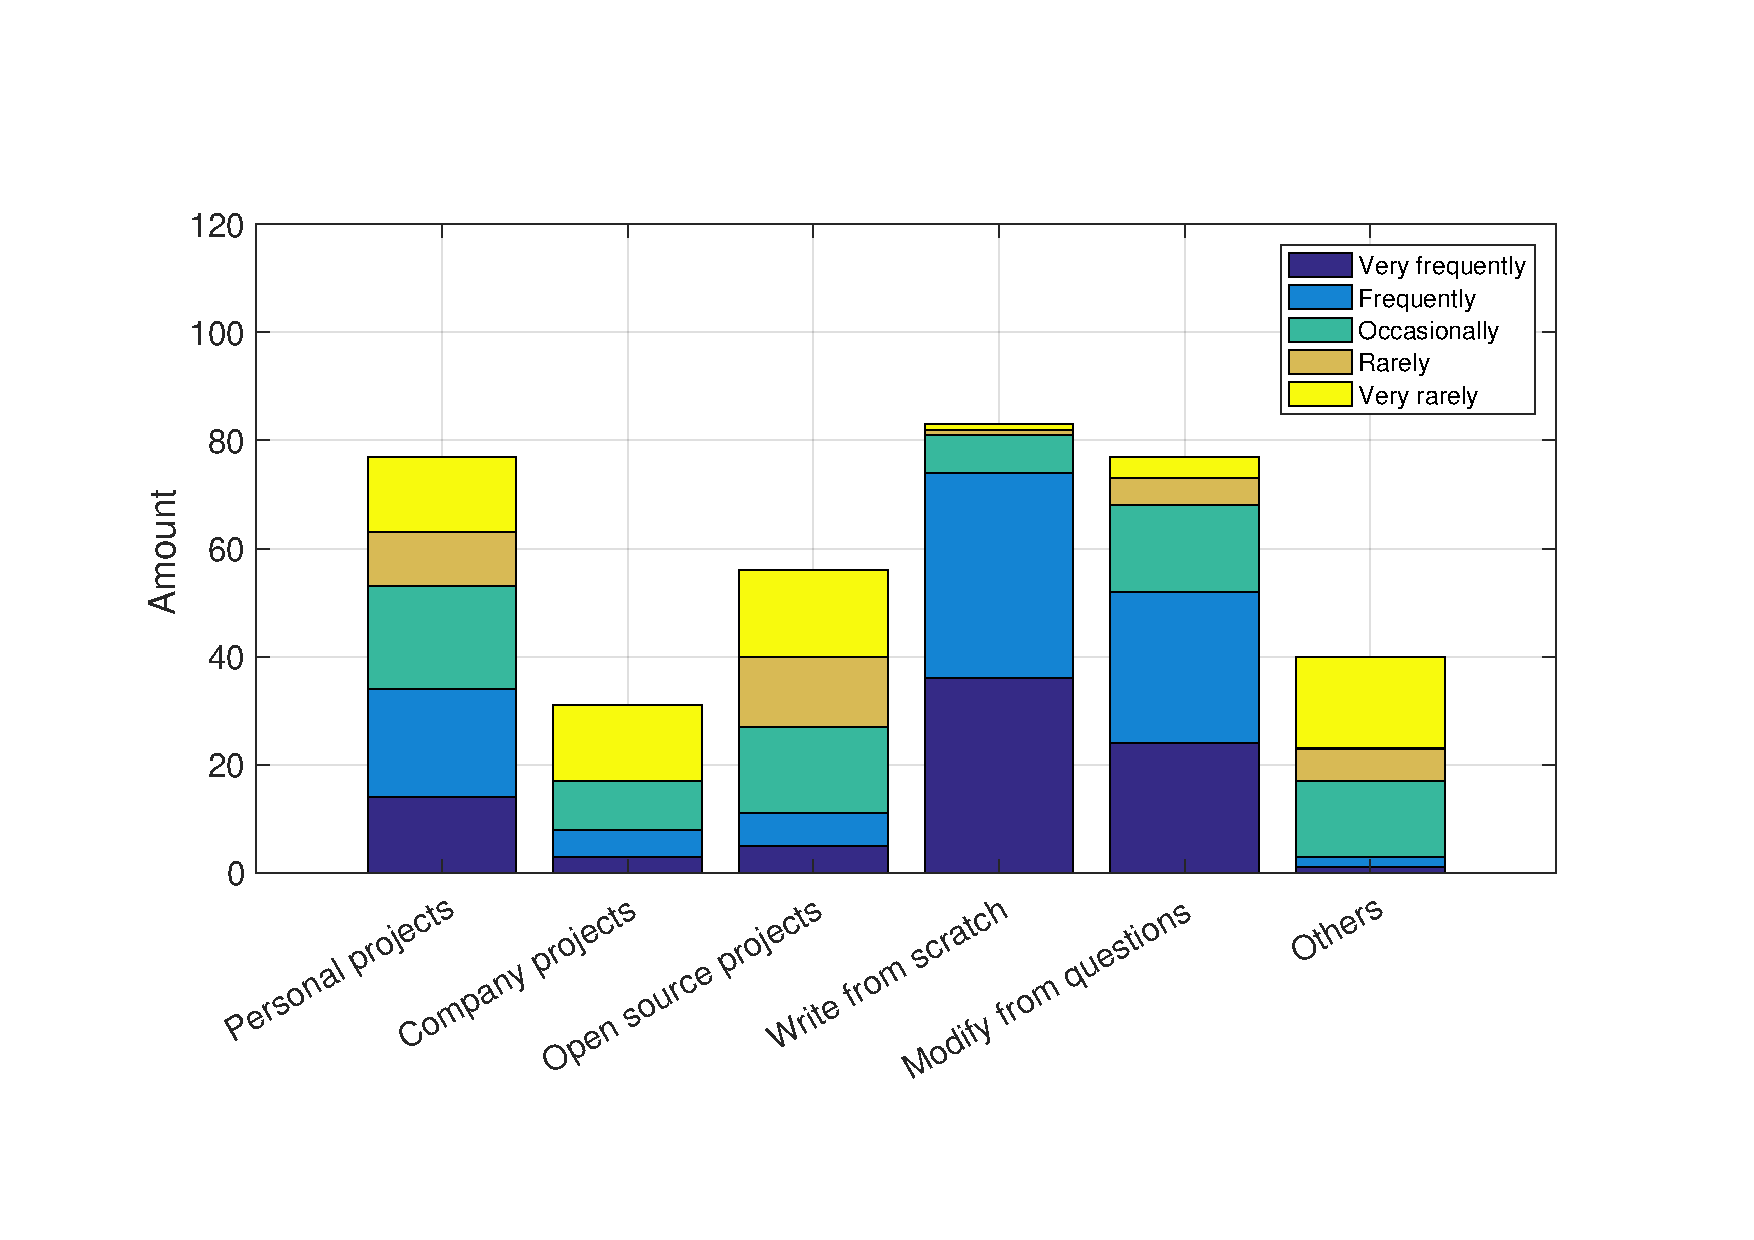
\includegraphics[width=0.9\linewidth]{survey_snippet_source}
	\caption{The sources of code snippets in Stack Overflow answers}
	\label{fig:survey_snippet_source}
\end{figure}

We asked the remaining 200 participants for the origins of code snippets in
their answers. We provided six locations including the answerer's personal
projects, the answerer's company projects, open source projects, writing the
code from scratch, copying and modifying the code from the question, and others
(e.g.,\ code that are copied from other questions or answers on Stack Overflow)
and we asked them to rate how often they copied the code from these locations. The
results are shown in \Cref{fig:survey_snippet_source}. Looking at the Very
Frequently section, we can see that the answerers mainly write new code from
scratch (106) or copy and modify the code snippets from the question for each answer (66),
while fewer numbers are from other sources including their personal projects
(28), their company projects (4), and open source projects (9). Although
copying from open source projects is not the most popular choice, the answerers
still rely on them sometimes. As shown in the figure, there are 14, 31, and 33
participants who frequently, occasionally, and rarely copied code snippets from
open source projects.

\vspace{0.25cm}
\textit{RQ 1.1 How often are Stack Overflow
	answerers aware of the outdated code and 
	licensing conflicts when
	they answer a question on Stack Overflow?} 
\vspace{0.25cm}

\textbf{Outdated Code Snippets:} We asked the answerers if they have ever been notified about outdated code in
their answers. 111 participants selected \textit{Yes} while the other 89 participants
selected \textit{No}. However, we found inconsistent results when we asked a follow-up
question on the frequency of being notified. As displayed in
\Cref{tab:survey_code_snippet_outdated}, the number of participants who have
\textit{Never} been notified about outdated code snippets in their answers drops
from 89 to 69.

\begin{table}
	\centering
	\caption{Notifications of outdated code snippets in answers}
	\label{tab:survey_code_snippet_outdated}
	\begin{tabular}{lrr}
		\toprule
		Notified of outdated code & Amount & Percent \\
		\midrule
		Very frequently (81--100\% of my answers) & 2 & 1\% \\
		Frequently (61--80\% of my answers) & 1 & 0.5\% \\
		Occasionally (41--60\% of my answers) & 9 & 4.5\% \\
		Rarely (21--40\% of my answers) & 16 & 8\% \\
		Very rarely (1--20\% of my answers) & 103 & 51.5\% \\
		Never (0\% of my answers) & 69 & 34.5\% \\
		\midrule
		Total & 200 & 100\% \\
		\bottomrule
	\end{tabular}
\end{table}

We found that although the answerers have been notified of outdated code in their
answers, for 51.5\% of them such notifications occur very rarely (only 1--20\%
of the answers). Only 3 participants reported that they were notified in more
than 60\% of their answers. This notification to the answerer can be done 
via several means, such as contacting the author directly or 
writing a comment saying that the answer is
already outdated.
The low percentage of outdated code notifications
reflect the experience of high reputation answerers who accumulate the reputation for a
long time. Due to the voting mechanism of Stack Overflow, high-reputation users
usually provide high-quality answers to earn upvotes from other users. They are
careful when posting code snippets in the answer to avoid problems and, vice versa, 
getting downvotes. It would be interesting to compare the findings to
Stack Overflow answerers who are newer and have a lower reputation. However, we
leave it to future work.

\begin{table}
	\centering
	\caption{Fixing of outdated code snippets in answers}
	\label{tab:survey_code_snippet_outdated_fix}
	\begin{tabular}{lrr}
		\toprule
		Fixing of outdated code & Amount & Percent \\
		\midrule
		Very frequently (81--100\% of the cases) & 48 & 36.6\% \\
		Frequently (61--80\% of the cases) & 27 & 20.6\% \\
		Occasionally (41--60\% of the cases) & 30 & 22.9\% \\
		Rarely (21--40\% of the cases) & 11 & 8.4\% \\
		Very rarely (1--20\% of the cases) & 8 & 6.1\% \\
		Never (0\% of the cases) & 7 & 5.3\% \\
		\midrule
		Total & 131 & 100.0\% \\
		\bottomrule
	\end{tabular}
\end{table}

We then asked 131 participants who have been notified of their outdated code a
follow-up question \textit{``how frequently did you fix your outdated code on Stack
	Overflow?''}. The answers, depicted in
\Cref{tab:survey_code_snippet_outdated_fix}, show that more than half of them
(57.2\%) very frequently or frequently fix the outdated code snippets. However,
there are 19.8\% of the answerers in both groups who rarely, very rarely, or never fix 
their outdated code.
%
%The responses from the answerers support our findings of outdated online code
%clones in RQ3. 

%\vspace{0.25cm}
%\textit{How often are Stack Overflow
%	answerers aware of licensing conflicts when
%	they answer a question on Stack Overflow?} 
%\vspace{0.25cm}

\begin{table}
	\centering
	\caption{Inclusion of software license in answer}
	\label{tab:survey_license_include}
	\begin{tabular}{lr}
		\toprule
		Include license? & Amount \\
		\midrule
		No. & 197 \\
		Yes, in code comment &	1 \\
		Yes, in text surrounding the code & 2 \\
		\midrule
		Total & 200 \\
		\bottomrule
	\end{tabular}
\end{table}

\textbf{The License of Code Snippets:} Among the 200 answerers who include code snippets in their answers, 124
answerers are aware that Stack Overflow applies Creative Commons
Attribution-ShareAlike 3.0 Unported (CC BY-SA 3.0) to content in the posts,
including code snippets, while the rest (76) are not. Nevertheless, as shown in
\Cref{tab:survey_license_include}, almost all of them (197) reported that they
did not include license statement in their code snippets due to several reasons.
First, some answerers chose to post only their own code or code that was adapted
from the question; hence they are automatically subjected to CC BY-SA 3.0.
Second, they copied the code from company or open source projects that they knew
were permitted to be publicly distributed. Third, some answerers believe that
code snippets in their answers are too small to claim any intellectual property
on them and fall under fair use~\cite{fairuse}.

While nobody explicitly includes a software license in their snippets,
many users include a statement on their profile page that all their
answers are under a specific license. For example, a Stack Overflow user includes 
the following text in his/her profile page.

\begin{quotation}
	\noindent \textit{All code posted by me on
		Stack Overflow should be considered public domain without copyright. For
		countries where public domain is not applicable, I hereby grant everyone the
		right to modify, use and redistribute any code posted by me on Stack Overflow
		for any purpose. It is provided ``as-is'' without warranty of any kind.}
\end{quotation}

Many users either declare their snippets to be public domain, or they grant
additional licenses, e.g.,\ Apache 2.0 or MIT/Expat.

\begin{table}
	\centering
	\caption{Checking for licensing conflicts with CC BY-SA 3.0}
	\label{tab:survey_license_check}
	\begin{tabular}{lrr}
		\toprule
		Check license conflicts? & Amount & Percent \\
		\midrule
		Very Frequently (81--100\% of the time)	& 14 & 7\% \\
		Frequently (61--80\% of the time) & 7 & 3.5\% \\
		Occasionally (41--60\% of the time) & 10 & 5\% \\
		Rarely (21--40\% of the time) & 16 & 8\% \\
		Very rarely (1--20\% of the time) & 15 & 7.5\% \\
		Never (0\% of the time) & 138 & 69\% \\
		\midrule
		Total & 200 & 100\% \\
		\bottomrule
	\end{tabular}
\end{table}

We asked the answerers a follow-up question of how frequently they checked for a
conflict between software license of the code snippets they copied to their
answers and Stack Overflow's CC BY-SA 3.0. As shown in
\Cref{tab:survey_license_check}, approximately 69\% of answerers did not perform
the checking. Nonetheless, there are about 10.5\% of the answerers who very
frequently or frequently check for licensing conflicts when they copy code
snippets to Stack Overflow.

%Similar to outdated code, the responses from the answerers support our findings
%of licensing conflicts in online code clones in RQ4 and possibly explain why most of
%the clones copied from open source projects and external sources do not include
%their original software license.

\begin{boxquote}
	To answer RQ 1.1, although most of the Stack Overflow answerers are aware that their code
	can be outdated, 51.5\% of the answerers were very rarely notified and 35.5\% have never been notified of
	outdated code in the answers. After being notified, 19.8\% of them rarely or never fix the outdated code.
	124 answerers out of 200 (62\%) are aware of Stack Overflow's
	CC BY-SA 3.0 license applied to code snippets in questions and answers. However,
	only 3 answerers explicitly include software license in their answers. Some 
	answerers choose to include the license in their profile page instead. 69\% of the
	answerers never check for licensing conflicts between their copied code snippets
	and Stack Overflow's CC BY-SA 3.0.
%	To answer RQ 1.1, although most of the Stack Overflow answerers are aware that their code
%	can be outdated, half of the answerers were very rarely notified of
%	outdated code in the answers. After being notified, some of them rarely or never fix the outdated code.
%	More than half of the answerers are aware of Stack Overflow's
%	CC BY-SA 3.0 license. Only 3 answerers explicitly include software license in their answers
%	while some of them choose to include the license in their profile page instead. More than half of the
%	answerers never check for licensing conflicts between their copied code snippets
%	and Stack Overflow's CC BY-SA 3.0.
\end{boxquote}

\textbf{Open Comments:} We also invited the participants to give a
free-form comment regarding their concerns about answering Stack Overflow with code
snippets. Besides the one we present earlier in the introduction, these are
interesting comments we received.

\begin{enumerate}
	\item \textit{``When I copy code it's usually short enough to be considered "fair
		use" but I am not a lawyer or copyright expert so some guidance from Stack Overflow would be
		helpful. I'd also like the ability to flag/review questions that violate these
		guidelines.''}
	\item \textit{``My only concern, albeit minor, is that I know people blindly copy
		my code without even understanding what the code does.''}
	\item \textit{``The main problem for me/us is outdated code, esp. as old answers
		have high google rank so that is what people see first, then try and fail. Thats
		why we're moving more and more of those examples to knowledge base and docs and
		rather link to those.''}
	\item \textit{``Lot of the answers are from hobbyist so the quality is poor.
		Usually they are hacks or workarounds (even MY best answer on Stack Overflow is a
		workaround).''}
\end{enumerate}

The comments highlight that Stack Overflow users are unsure about the
legal implications of copying code, that code is copied without
understanding it, and that the quality of code on Stack Overflow is
often low.

\subsubsection{The Visitor Survey}

We received answers from 89 participants. Two participants never copy code from
Stack Overflow, so we analysed the answers of the remaining 87 participants. We
only present a summary of the survey answers in this paper, and the full
analysis is available as a research note~\cite{Ragkhitwetsagul_RN2017}.

\textbf{General Information: }
Twenty-four (27\%) and twenty-one (24\%) participants have over 10 years and 5--10
years of experience respectively. There are 19 participants (21\%) who have 3--5
years, 18 (20\%) who have 1-2 years, and 7 (8\%) participants who have less than a
year of programming experience.

\textbf{The Choice for programming solutions: }
Stack Overflow is ranked higher than official documentation, online
repositories, and books as the resource to look for programming solutions.
Developers rely on Stack Overflow answers because they are easy to search for on
the web. Moreover, 64\% of the participants reuse code snippets from Stack
Overflow at least once a week. They copy code from Stack Overflow because they
can be found easily from a search engine, solve similar problems to their
problems, provide helpful context, and offer voting mechanism and accepted answers. 

\vspace{0.25cm}
\textit{RQ 1.2 How often do Stack Overflow
	visitors experience the outdated code and licensing conflicts when
	they reuse code in an answer from Stack Overflow?}
\vspace{0.25cm}

\begin{table}
	\centering
	\caption{Problems from Stack Overflow code snippets}
	\label{tab:visitor_survey_code_problems}
	\begin{tabular}{lr}
		\toprule
		Problem & Amount \\
		\midrule
		Mismatched solutions & 40 \\
		Outdated solutions & 39 \\
		Incorrect solutions	& 28 \\
		Buggy code & 1 \\
		\bottomrule
	\end{tabular}
\end{table}

\begin{table}
	\centering
	\caption{Frequency of reporting the problems to Stack Overflow posts}
	\label{tab:visitor_survey_report_problem}
	\begin{tabular}{lrr}
		\toprule
		Report? & Amount & Percent \\
		\midrule
		Very Frequently (81--100\% of the time)	& 1 & 1.8\% \\
		Frequently (61--80\% of the time) & 1 & 1.8\% \\
		Occasionally (41--60\% of problematic snippets) & 3 & 5.3\% \\
		Rarely (21--40\% of problematic snippets) & 8 & 14.0\% \\
		Very rarely (1--20\% of problematic snippets) & 8 & 14.0\% \\
		Never (0\% of problematic snippets) & 36 & 63.2\% \\
		\midrule
		Total & 57 & 100\% \\
		\bottomrule
	\end{tabular}
\end{table}

The survey results show that 57 out of 87 Stack Overflow visitors encountered a
problem from reusing Stack Overflow code snippets. Ten participants experienced
problems for more than 80\% of the copied snippets, and sixteen participants
faced problems for 40--60\% of the reused code. As shown in~\Cref{tab:visitor_survey_code_problems}, 
the problems ranked by frequency
include mismatched solutions (40), outdated solutions (39), incorrect solutions
(28), and buggy code (1). Sixty-three percent of the participants never report
the problems back to Stack Overflow (\Cref{tab:visitor_survey_report_problem}). 
The ways of reporting the problems
(22 answers) included down-voting the answer containing the problematic code
snippet (8), writing a comment saying that the code has problems (10),
contacting the answerers regarding the problems directly (2), and posting a
better snippet as new answer on same topic (2).

\begin{table}
	\centering
	\caption{Check for licensing conflicts before using Stack Overflow snippets}
	\label{tab:visitor_survey_license_check}
	\begin{tabular}{lrr}
		\toprule
		License check? & Amount & Percent \\
		\midrule
		Very frequently (81--100\% of the time) & 0 & 0.0\% \\
		Frequently (61--80\% of the time) & 7 & 8.1\%
\\
		Occasionally (41--60\% of the time) & 6 & 6.9\%
\\
		Rarely (21--40\% of the time) & 6 & 6.9\% \\
		Very rarely (1--20\% of the time) & 11 & 12.6\% \\
		Never (0\% of the time)	& 57 & 65.5\% \\
		\midrule
		Total & 87 & 100\% \\
\bottomrule
\end{tabular}
\end{table}

In addition, 74 out of the 87 (85\%) participants are not
aware of Stack Overflow CC BY-SA 3.0 license, and 62\% never give attributions to
the Stack Overflow posts they copied the code snippets from. 
As shown in \Cref{tab:visitor_survey_license_check}, we found that 66\%
of the visitors never check for software licensing conflicts between Stack
Overflow code snippets and their projects. Interestingly, 9\% of the
participants encountered legal issues. Due to the anonymity of
the survey, we could not investigate further regarding the legal issues that the
participants faced from using Stack Overflow code snippets.
To the best of our
knowledge, a study of legal problems from reusing Stack Overflow code snippets
has never been done before and will be our future work.

%The visitors survey confirms the findings from the previous studies that Stack
%Overflow code snippets can be problematic~\cite{Zhang2018,Acar2016,An2017,Fischer2017}. 
%Sixty-six
%percent of the visitors experienced a problem from reusing Stack Overflow code
%snippets ranging from incorrect solutions, outdated solutions, mismatched
%solutions, to buggy code. Although they are aware of the problems, half of them
%(56\%) never reports back to the Stack Overflow discussions. On the other hand,
%the visitors rarely give attributions to Stack Overflow when they reuse code
%snippets from the website, similar to the findings reported
%by~\cite{Baltes2017}. The visitors are generally not aware of the CC BY-SA 3.0
%license, and more than half of them never check for license compatibility when
%reusing Stack Overflow code snippets. 
%Sixty-nine Stack Overflow visitors (79\%) who adopted code from Stack Overflow never 
%check if the code snippet originated from a different source (e.g.,~an open source project) 
%and if they had an incompatible license to their projects.
%Moreover, we also found that 9\% of the participants
%encountered legal issues by copying code from Stack Overflow.

\begin{boxquote}
	To answer RQ 1.2, Stack Overflow visitors experienced several issues from Stack
Overflow answers including outdated code. 85\% of them are not aware of
CC BY-SA 3.0 license enforced by Stack Overflow and 66\% never check for license
conflicts when reusing code snippets.
\end{boxquote}

\subsection{RQ2: Online Code Clones} 
\vspace{0.25cm}
\textit{To what extent is source
	code cloned between Stack Overflow and open source projects?}
\vspace{0.25cm}

The statistics on clones obtained from the merged clone data set are
presented in~\Cref{tab:snippets}. Simian and SourcererCC
reported clones in 460 snippets, approximately 0.6\% of the
72,365 Stack Overflow snippets, associated with 59 Qualitas
projects. For the cloned Stack Overflow snippets, the
average ratio of cloned code is 53.28\% (i.e.,\ the number of cloned
lines of the cloned Stack Overflow snippet).

\begin{table}
	\caption{Investigated online clone pairs and corresponding snippets
		and Qualitas projects}
	\label{tab:snippets}
	\centering
	\begin{tabular}{p{2.2cm}rrrr}
		\toprule
		Set & Pairs & Snippets & Projects & Cloned ratio \\
		\midrule
		Reported clones & 2,289 & 460 & 59 & 53.28\% \\ 
		\midrule
		TP from manual validation & 2,063 & 443 & 59 & 54.09\% \\ 
		\bottomrule
	\end{tabular}
\end{table}

Lastly, during the manual investigation of 2,289 clone pairs, we identified 226 pairs
as not clones (NC), i.e.,~false positives. After removing
them, the set still contains 2,063 true positive clone pairs between 443 Stack
Overflow snippets and 59 Qualitas projects. The average cloned ratio for the
true positive clone pairs is 54.09\%.

\begin{boxquote}
	To answer RQ2, we found 2,063 manually confirmed clone pairs between 443 Stack Overflow code snippets
	and 59 Qualitas proejcts. 
	%After the manual confirmation, 2,076 pairs as true positives, i.e.,~
	%they are manually confirmed as clones, which 
	%account for 59 Qualitas projects and
	%443 Stack Overflow code snippets.
\end{boxquote}

\subsection{RQ3: Patterns of Online Code Cloning}
\vspace{0.25cm}
\textit{How do online code clones occur?}
\vspace{0.25cm}

We performed a manual classification
of the 2,289 merged clone pairs by following the classification process
in \Cref{fig:classification_process}. 
The classification results are shown in \Cref{tab:classification_good_o} 
and explained in the following.

\begin{table*}
	\centering
	\caption{Classifications of online clone pairs.}
	\label{tab:classification_good_o}
	%\small
	%\resizebox{\columnwidth}{!}
\end{table*}

%\begin{table}
%	\centering
%	\caption{Statistics of clone sizes}
%	\label{tab:clone_stats}
%	\begin{tabular}{lrrrr}
%		\toprule
%		Clones & Min & Max & Mean & Median \\
%		\midrule
%		QS & 10 & 135 & 18.6 & 14 \\
%		SQ & 21 & 21 & 21.0 & 21 \\
%		UD & 10 & 104 & 18.1 & 14 \\
%		EX & 10 & 48 & 16.7 & 14 \\
%		BP & 10 & 55 & 19.9 & 21 \\
%		IN & 11 & 22 & 13.8 & 13.0 \\
%		\bottomrule
%	\end{tabular} 
%\end{table}

\textbf{QS: Qualitas $\rightarrow$ Stack Overflow.} We found 247 online clone
pairs with evidence of cloning from Qualitas projects to Stack Overflow.
However, we observed that, in some cases, a cloned code snippet on Stack
Overflow matched with more than one code snippet in Qualitas projects because of
code cloning inside Qualitas projects themselves. To avoid double counting of
such online clones, we consolidated multiple clone pairs having the same Stack
Overflow snippet, starting line, and ending line into a single clone pair. We
finally obtained 153 QS pairs (\Cref{tab:classification_good_o}) having unique Stack Overflow code snippets and
associated with 23 Qualitas projects listed in \Cref{tab:qs_qualitas_projects}.
The most cloned project is \textsf{hibernate} with 23
clone pairs, followed by \textsf{eclipse} (21 pairs), \textsf{jung2} (19 pairs),
\textsf{spring} (17 pairs), and \textsf{jfreechart} (13 pairs). The clones are
used as examples and are very similar to their original Qualitas code with
limited modifications. Most of them have a statement in the Stack Overflow post
saying that the code is ``copied,'' ``borrowed'' or ``modified'' from a specific
file or class in a Qualitas project. For example, according to the motivating
example in \Cref{fig:before-after}, we found evidence in the Stack Overflow Post
22315734 saying that \textit{``Actually, you can learn how to compare in Hadoop
from WritableComparator. Here is an example that borrows some ideas from it.''}

\begin{table}
	\centering
	\caption{Qualitas projects associated with QS and UD online clone pairs}
	\label{tab:qs_qualitas_projects}
	%\small
	%\resizebox{\columnwidth}{!}{%
	\begin{tabular}{lrlr}
		\toprule
		\multicolumn{2}{c}{QS} & \multicolumn{2}{c}{UD} \\
		\midrule
		Project & Pairs & Project & Pairs\\
		\midrule
		hibernate & 23 & netbeans & 11 \\
		eclipse & 21 & eclipse & 8 \\
		jung2 & 19 & jstock & 5 \\
		spring & 17 & compiere & 5 \\
		jfreechart & 13 & ireport & 4 \\
		hadoop & 10 & jmeter & 4 \\
		tomcat & 8 & jung2 & 3 \\
		log4j & 8 & jhotdraw & 3 \\
		struts2 & 5 & c-jdbc & 3 \\
		weka & 4 & log4j & 3 \\
		lucene & 4 & wct & 2 \\
		poi & 3 & hibernate & 2 \\
		junit & 3 & tomcat & 2 \\
		jstock & 2 & spring & 1 \\
		jgraph & 2 & rssowl & 1 \\
		jboss & 2 & mvnforum & 1 \\
		jasperreports & 2 & jfreechart & 1 \\
		compiere & 2 & jboss & 1 \\
		jgrapht & 1 & hadoop & 1 \\
		itext & 1 & geotools & 1 \\
		c-jdbc & 1 & freemind & 1 \\
		ant & 1 & findbugs & 1 \\
		antlr4 & 1 & cayenne & 1 \\
		\bottomrule
	\end{tabular} 
	%}
\end{table}

We analysed the time it took for the clone to appear from Qualitas
projects to Stack Overflow. The clone ages were calculated by counting the
number of months between the date of each Qualitas project and the date the answer
was posted on Stack Overflow as shown in~\Cref{fig:boxplotcloneage}.
We found that, on average, it took the clones around 2 years since they appeared
in Qualitas projects to appear on Stack Overflow answers. Some of the clones
appeared on Stack Overflow almost at the same time as the original, while the
oldest clones took around 5 years.

\begin{figure}
	\centering
	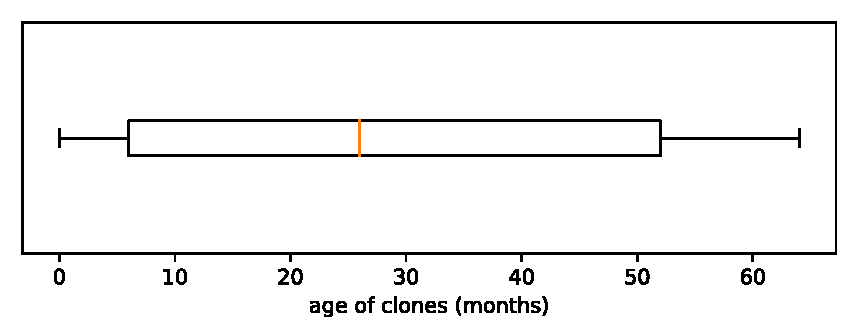
\includegraphics[width=0.9\linewidth]{boxplot_clone_age}
	\caption{Age of QS online code clones.}
	\label{fig:boxplotcloneage}
\end{figure}

\textbf{SQ: Stack Overflow $\rightarrow$ Qualitas.} We found one pair with
evidence of cloning from Stack Overflow post ID 698283 to
{\small\texttt{POIUtils.java}} in \textsf{jstock} project. The user
 who asked the question on Stack Overflow is an author of
\textsf{jstock}. The question is about determining the right method to call
among 7 overloading methods of {\small\texttt{setCellValue}} during runtime. We
could not find evidence of copying or attribution to Stack Overflow in
\textsf{jstock}. However, considering that the 25 lines of code of
{\small\texttt{findMethodToInvoke}} method depicted in \Cref{fig:jstock_code} in Stack
Overflow is very similar to the code in \textsf{jstock} including comments, it is almost certain that
the two code snippets form a clone pair. In addition, the Stack Overflow answer was
posted on March 30, 2009, while the code in {\small\texttt{POIUtils}} class in
\textsf{jstock} was committed to GitHub on the next day of March 31, 2009.

\begin{figure}
	\begin{lstlisting}
private Method findMethodToInvoke(Object test) {
  Method method = parameterTypeMap.get(test.getClass());
  if (method != null) {
    return method;
  }

  // Look for superclasses
  Class<?> x = test.getClass().getSuperclass();
  while (x != null && x != Object.class) {
    method = parameterTypeMap.get(x);
    if (method != null) {
      return method;
    }
    x = x.getSuperclass();
  }

  // Look for interfaces
  for (Class<?> i : test.getClass().getInterfaces()) {
    method = parameterTypeMap.get(i);
    if (method != null) {
      return method;
    }
  }
  return null;
}
	\end{lstlisting}\vspace{-2ex}
	\caption{The {\small\texttt{findMethodToInvoke}} that is found to be copied from Stack Overflow post 698283 to {\small\texttt{POIUtils}} class in \textsf{jstock}.}
	\label{fig:jstock_code}
\end{figure}

This very low number of SQ clone pair is very likely due to the age of the
Qualitas corpus as another study~\cite{An2017} showed the presence of clones
from Stack Overflow in newer open source data sets. This is expected and
comes from our experimental design since
we are more interested in cloning from Qualitas to Stack Overflow.

\begin{figure}
	\centering
	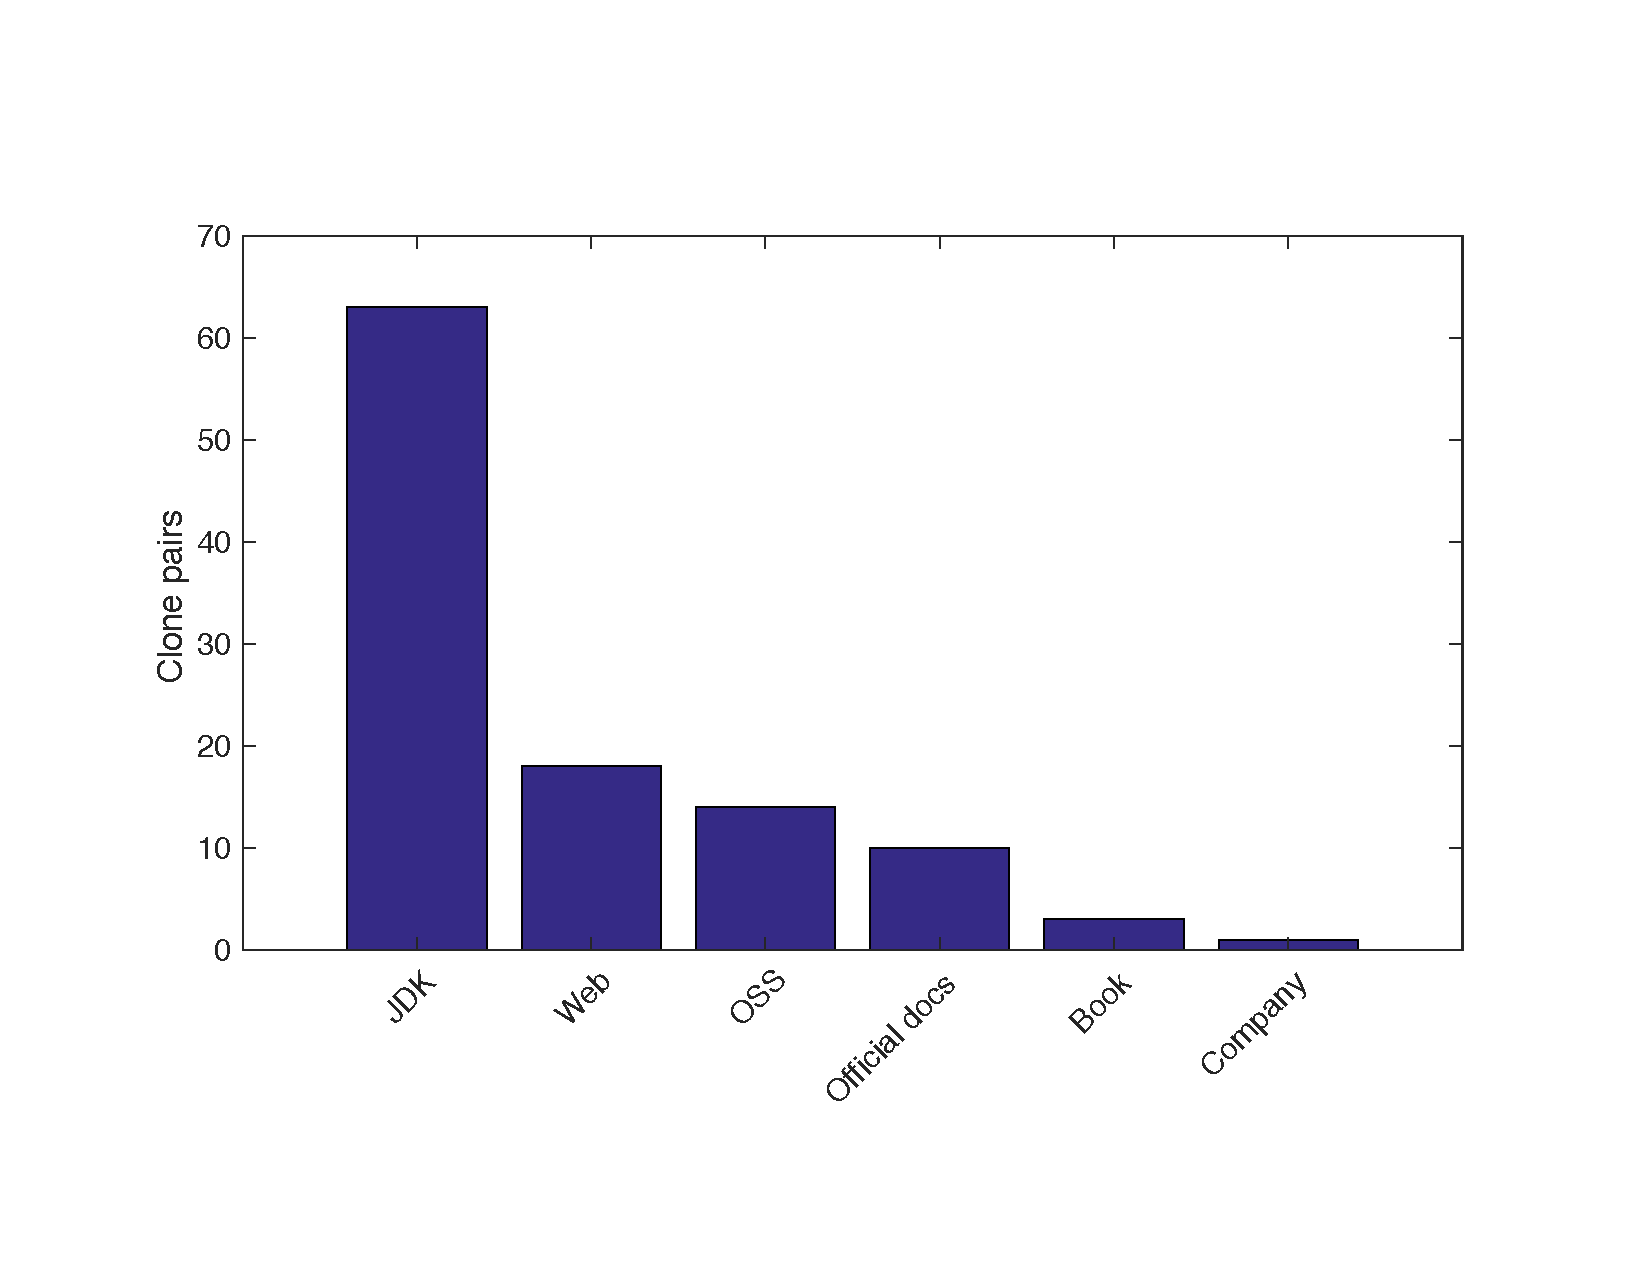
\includegraphics[width=0.9\linewidth]{ex_sources}
	\caption{Original sources of EX clone pairs}
	\label{fig:ex_sources}
\end{figure}

\textbf{EX: External Sources.} We found 197 clone pairs from external sources to
Stack Overflow. After consolidating duplicated SO snippets due to multiple
intra-clone instances in Qualitas, we obtained 109 EX pairs. We found
evidence of copying from an external source to both Stack
Overflow and Qualitas in 49 pairs. Each of the pairs contains
statement(s) pointing to the original external location of the cloned
code in Qualitas and Stack Overflow. Besides, we found evidence
of copying from an external source to Stack Overflow, but not in
Qualitas, in 60 pairs. 
Our
analysis shows that the external sources fall into six groups as displayed in
\Cref{fig:ex_sources}. There are 63 EX online clone pairs copied
from source code of Java SDK (e.g.,\ \textsf{java.util}, \textsf{javax.swing}, \textsf{javax.servlet}), 
18 pairs from websites, 14 pairs from open
source systems not in Qualitas (e.g.,\ \textsf{Mozilla
	Rhino}), 10 pairs from Java official documentation by Sun
Microsystems or Oracle, 3 pairs from books, and 1 pair from a company
project. For example, Stack Overflow Post 9549009 contains a code comment saying
\textit{``Copied shamelessly from
	org.bouncycastle.crypto.generators.PKCS5S2ParametersGenerator''} which is an
open source project not included in the Qualitas corpus. Post 92962 includes a {\small\texttt{VerticalLabelUI}}
class with a license statement showing that it is developed by a private company
called \textsf{Sapient}. Post 12879764 has a text saying \textit{``Code modified
	and cleaned from the original at Filthy Rich Clients.''} which is a book for
developing animated and graphical effects for desktop Java applications. Another
example is a copy of the code from a website in post 15260207. The text surrounding
source code reads ``\textit{I basically stole this from the web and modified it
	slightly... You can see the original post here
	(\url{http://www.java2s.com/Code/Java/Swing-JFC/DragListDemo.htm}).}''.
Interestingly, the code is actually a copy from Sun Microsystems.

These findings complement a study of clones between software
projects~\cite{Svajlenko2014}. We found that cloning can also happen among
different sources on the Internet just like software projects. There are 18 clone
pairs that originated from programming websites including \url{www.java2s.com}
and \url{exampledepot.com}. Moreover, there is one snippet which comes from a
research website. We found that a snippet to generate graphical \textit{Perlin
	noise} is copied from NYU Media Research Lab
(\url{http://mrl.nyu.edu/~perlin/noise/}) website and is used in both Stack Overflow
answer and the \textsf{aoi} project with attribution. 

%There are other EX pairs which
%are copied from open source libraries or Java SDK such as \textsf{Mozilla
%	Rhino}, \textsf{java.util}, \textsf{javax.swing}, \textsf{javax.servlet}, and
%the \textsf{bouncycastle} cryptography project.

\textbf{UD: Unknown Direction.} We found 107 online clone pairs, reduced to 65
pairs after consolidating the clones, with no evidence of cloning between Qualitas
and Stack Overflow but with a high code similarity that suggests cloning. 
The most cloned project is \textsf{netbeans} with 11 clone pairs. Most of the
clones are a large chunk of code handling GUI components. Although these GUI
clones might be auto-generated by IDEs, we did not find any evidence. The second
most cloned project is \textsf{eclipse} (8 pairs), followed by
\textsf{jstock}  (5 pairs),
a free stock market software, and \textsf{compiere}, a customer
relationship management (CRM) system.

\textbf{BP: Boiler-Plate.} There were a large amount of boiler-plate clone pairs
found in this study. We observed 1,495 such clone pairs and 216 after
consolidation. The BP clone pairs account for 65\% of all clone pairs we
classified. The majority of them are {\small{\texttt{equals()}}} methods.

\textbf{IN: Inheritance/interface.} There were 16 clone pairs, 9 pairs after
consolidation, found to be similar because they implement the same interface or
inherit from the same class. An example is the two implementations of a
custom data type which implements {\small\texttt{UserType}}. They share similar
{\small\texttt{@Override}} methods of {\small\texttt{deepCopy}},
{\small\texttt{isMutable}}, {\small\texttt{assemble}},
{\small\texttt{disassemble}}, and {\small\texttt{replace}}.

\textbf{NC: Not Clones.} There were 226 non-clone
pairs, 53 after consolidation. Mainly, they are false positive clones caused by code
normalisation and false type-3 clones from SourcererCC. 
Examples of the NC clone instances include {\small\texttt{finally}} or
{\small\texttt{try-catch}} clauses that were accidentally the same due
to their tiny sizes, and similar {\small\texttt{switch-case}}
statements.

\begin{boxquote}
To answer RQ3, we found 153 pairs with
strong evidences to be cloned from 23 Qualitas projects to Stack Overflow, 1 pair
was cloned from Stack Overflow to Qualitas, and
109 pairs were found to be cloned to Stack Overflow from external
sources. However, the largest amount of the clone pairs
between Stack Overflow and Qualitas projects are \linebreak boiler-plate code
(216), followed by 65 clone pairs with no evidence that the code has actually been copied,
and 9 pairs of clones due to implementing the same interface or inheriting the same class.
\end{boxquote}

\subsection{RQ4: Outdated Online Code Clones}
\vspace{0.25cm}
\textit{Are online code clones up-to-date compared to their counterparts in the original projects?}
\vspace{0.25cm}

\begin{figure*}
	\centering
	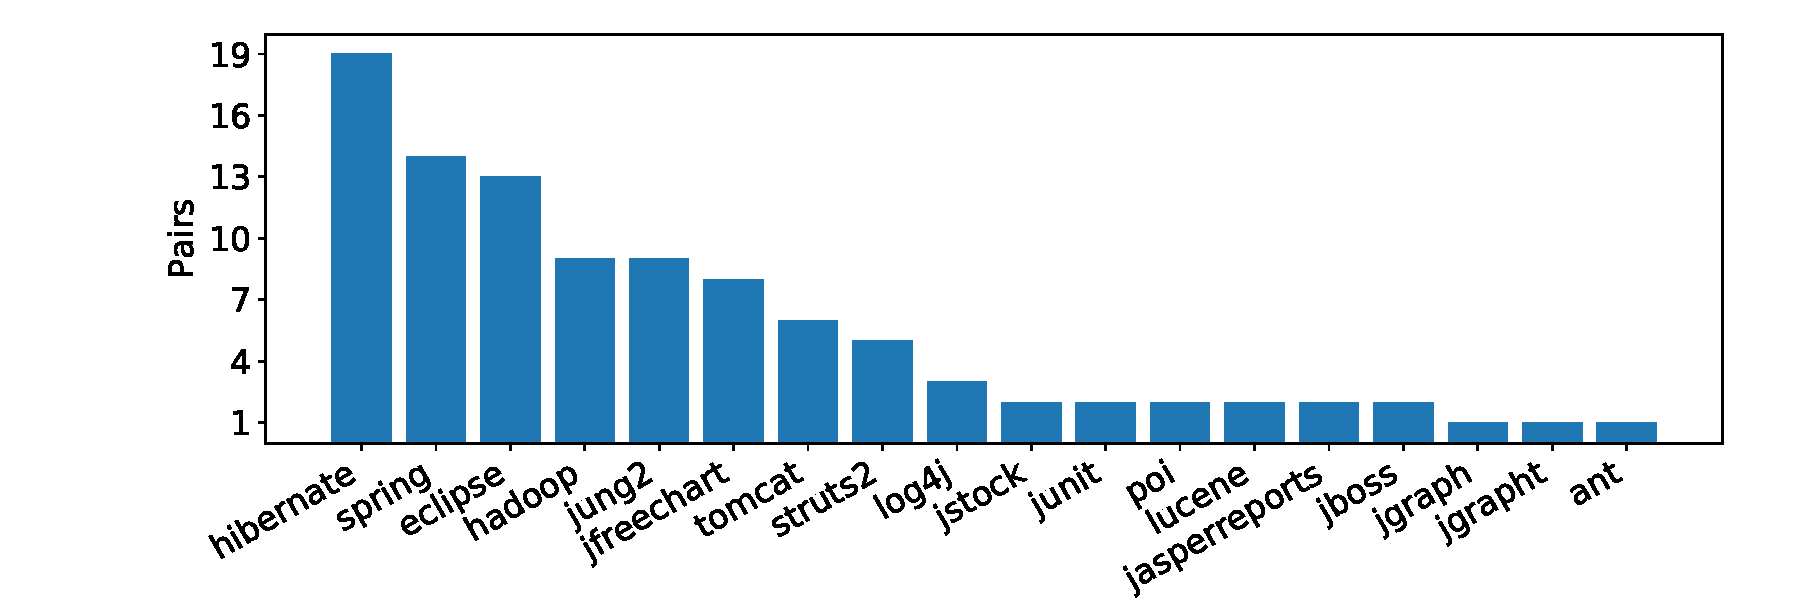
\includegraphics[width=0.8\linewidth]{outdated}
	\caption{Outdated QS online clone pairs group by projects}
	\label{fig:outdated}
\end{figure*}

We discovered 100 outdated online clone pairs out of 153 pairs. As shown in
\Cref{fig:outdated}, \textsf{hibernate} has the highest number of 19 outdated
pairs, followed by 14 from \textsf{spring}, 13 from \textsf{eclipse}, and 9 from
\textsf{hadoop}. Besides the two examples of outdated code in % \textsf{hadoop}'s
{\small{\texttt{WritableComparator}}} and
{\small{\texttt{StringUtils}}} class from \textsf{hadoop} shown in
\Cref{fig:before-after} and \Cref{fig:before-after_2}, we also found a few
outdated code elements which contained a large number of modifications. For
example, the code snippet in Stack Overflow post 23520731 is a copy of
{\small{\texttt{SchemaUpdate.java}}} in \textsf{hibernate}. The code has been
heavily modified on February 5, 2016.

%\begin{figure}
%	\centering
%	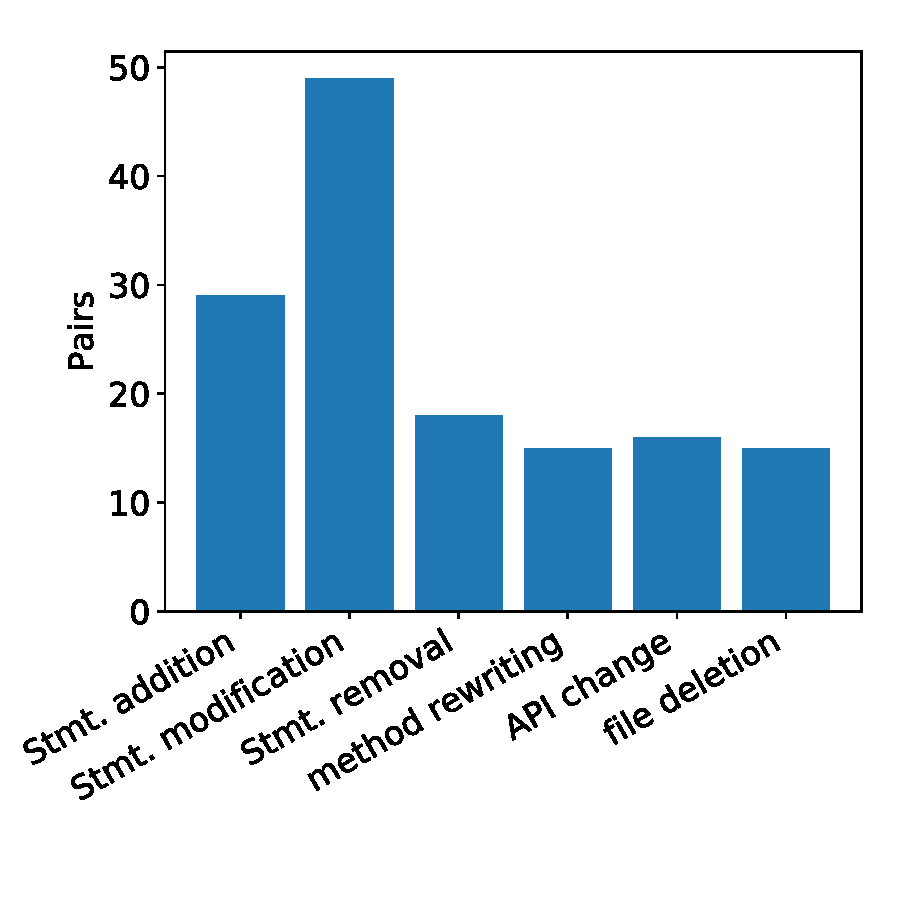
\includegraphics[width=0.7\linewidth]{mod_types}
%	\caption{Six code modification types found when comparing the outdated clone pairs to their latest versions}
%	\label{fig:mod_types}
%\end{figure}

\begin{table}
	\centering
	\caption{Six code modification types found when comparing the outdated clone pairs to their latest versions}
	\label{tab:mod_types}
		\begin{tabular}{lr}
			\toprule
			Modification & Occurrences \\
			\midrule
			Statement modification & 50 \\
			Statement addition & 28 \\
			Statement removal & 18 \\
			Method signature change & 16 \\
			Method rewriting & 15 \\
			File deletion & 14 \\
			\bottomrule 
		\end{tabular}
\end{table}

We analysed code modifications which made Stack Overflow code outdated by going
through commits and git blame information. The six code modification
types found in the 100 outdated online clone pairs are summarised in
\Cref{tab:mod_types}. They include statement addition, statement modification,
statement removal, method rewriting, API change (changing in method signature),
and file deletion. We occasionally found multiple code modifications applied to
one clone pair at the same time but at a different location. The most often code
change found is statement modification (50 occurrences), followed by statement
addition (28 occurrences), statement removal (18 occurrences), change of
method signature, i.e.,~API change (16 occurrences), and method rewriting (15
occurrences). Moreover, in the 100 outdated pairs, we found 14 ``dead''
snippets. These snippets cannot be located in the latest version of the
projects. For example, the snippet in Stack Overflow post 3758110, a copy of
{\small{\texttt{DefaultAnnotationHandlerMapping.java}}} in \textsf{spring}, was
deleted in the commit
{\small{\texttt{02a4473c62d8240837bec297f0a1f3cb67ef8a7b}}} on
January 20, 2012, two years after it was posted.

\begin{table*}
	\centering
	\caption{Examples of the outdated QS online clones}
	\label{tab:stale_code_details}
	\resizebox{\linewidth}{!}{
		\begin{tabular}{cc|lcp{4cm}@{}rrc|lc@{}c}
			\toprule
			\multicolumn{2}{c|}{Stack Overflow} & \multicolumn{6}{c|}{Qualitas} & \multicolumn{3}{c}{Changes} \\ 
			\midrule
			Post & Date & Project & Ver. & File & Start & End & Date & Issue ID & Type$^*$ & Date \\
			\midrule
			2513183 & 25-Mar-10 & eclipse & 4.3 & GenerateToStringAction.java & 113 & 166 & 5-Jun-13 & Bug 439874 & \textit{S} & 17-Mar-15 \\
			22315734 & 11-Mar-14 & hadoop & 1.0.0 & WritableComparator.java & 44 & 54 & 25-Aug-11 & HADOOP-11323 & \textit{S} & 20-Nov-14 \\
			23520731 & 7-May-14 & hibernate & 4.2.2 & SchemaUpdate.java & 115 & 168 & 22-May-13 & HHH-10458 & \textit{S} & 5-Feb-16 \\
			18232672 & 14-Aug-13 & log4j & 1.2.16 & SMTPAppender.java & 207 & 228 & 31-Mar-10 & Bug 44644 & \textit{R} & 18-Oct-08 \\ 
			17697173 & 17-Jul-13 & lucene & 4.3.0 & SlowSynonymFilterFactory.java & 38 & 52 & 6-Apr-13 & LUCENE-4095 & \textit{D} & 31-May-12 \\
			21734562 & 12-Feb-14 & tomcat & 7.0.2  & FormAuthenticator.java & 51 & 61 & 4-Aug-10 & BZ 59823 &\textit{R} & 4-Aug-16 \\
			12593810 & 26-Sep-12 & poi & 3.6 & WorkbookFactory.java & 49 & 60 & 7-Dec-09 & 57593 & \textit{R} & 30-Apr-15 \\
			8037824 & 7-Nov-11 & jasperreports & 3.7.4 & JRVerifier.java & 1221 & 1240 & 31-May-10 & N/A & \textit{D} & 20-May-11 \\
			3758110 & 21-Sep-10 & spring & 3.0.5  & DefaultAnnotation\newline HandlerMapping.java & 78 & 92 & 20-Oct-10 & SPR-14129 & \textit{D} & 20-Jan-12 \\
			14019840 & 24-Dec-12 & struts & 2.2.1 & DefaultActionMapper.java & 273 & 288 & 17-Jul-10 & WW-4225 & \textit{S} & 18-Oct-13 \\
			\bottomrule 
			\multicolumn{10}{l}{{\footnotesize * \textit{S}:
					modified/added/deleted statements, \textit{D}: file
					has been deleted,  \textit{R}: method has been
					rewritten completely}}
		\end{tabular} %
	}
\end{table*}

Moreover, using the information in git commit messages, we can associate each
change to its respective issues in an issue tracking system, such as Bugzilla or
Jira. We found that in 58 cases, the cloned code snippets on Stack Overflow were
changed because of a request in the issue tracking system. Since issue tracking
systems are also used, besides bug reports, for feature request and feature
enhancements, having an issue tracking ID can reflect that most of the changes are important
and not only a superficial fix such as code formatting. The intent behind
the changes are grouped into six categories as shown in \Cref{tab:intent_outdated}.
Enhancement is the majority intent accounting for 65 of the 100 outdated code (65\%). 
Next is code deprecation (15\%), which represents the code snippets that are outdated due to the use of
deprecated functions or APIs. The code snippets that we analysed contained a few deprecated code statements while
the newest version (based on the time we did the analysis) of the same code
snippets no longer contain the deprecated part.
There were 10 outdated code snippets (10\%) caused by bug fixing.
They contained buggy code statements, and were later fixed in the newest version.
The rest of the changes are because of code refactoring (6\%), changing coding style (3\%), and 
the data format change (2\%).
Not all outdated code is toxic. 
However, the 10 buggy and outdated code snippets we found are toxic and are harmful to reuse.

\begin{table}
	\centering
	\caption{Intents of code changes in the 100 outdated code snippets}
	\label{tab:intent_outdated}
	\begin{tabular}{llr}
		\toprule
		Intent & Detail & Amount \\
		\midrule
		Enhancement & Add or update existing features & 64 \\
		Deprecation & Delete dead/deprecated code & 15 \\
		Bug & Fix bugs & 10 \\
		Refactoring & Refactor code for better design & 6 \\
		Coding style & Update to a new style guideline & 3 \\
		Data change & Changes in the data format & 2 \\
		\bottomrule
	\end{tabular}
\end{table}


\Cref{tab:stale_code_details} shows examples of the outdated online clones on
Stack Overflow. The table displays information about the clones from both Stack
Overflow and Qualitas side including the dates. We summarise the changes that
make the clones outdated into three types, modified/added/deleted statements
(\textit{S}), file deletion (\textit{D}), and method rewriting (\textit{R}),
along with the issue tracking number and the date of the change. The complete set of
100 outdated online clones can be found on the study website.

We performed a detailed investigation of the 100 outdated answers on Stack
Overflow, on May 6, 2018, approximately two years after the snapshot we analysed was created
to look for any changes, warnings, or mitigations made to the outdated code snippets.
We investigated the answers on three aspects: newer answers, higher-voted answers, and comments on the
outdated answers.\footnote{We also found that the Stack Overflow question ID 22262310, which has an outdated answer from \texttt{WritableComparator.java} (\Cref{fig:before-after}), has a negative score of -1. It is interesting to see if the negative score for the question impacts both the number of views and the trust that people place in the answer to a down-voted question. However, it is out of the scope of this study so we leave it as future work.} We found
34 posts which contained newer answers and 5 posts which contained answers with a higher number of
votes than the outdated answers. However, 99 of the 100 outdated answers were still
marked as accepted answers. For the comments, we check if there is any comment
to mitigate or point out the toxicity of the outdated code snippets. We found
that, out of 100 answers, 6 answers had a comment saying the
code in the answer is outdated or containing issues, such as \textit{``spring
	3.1 stuff''}, \textit{``...tried this but having connect exception --
	\texttt{javax.mail.MessagingException}:\textit{ Could not connect to SMTP host:
	\texttt{smtp.gmail.com}, port: 465''}, ``You should add a \texttt{buffer.reset(null, 0, 0);} at the end of the try block to avoid excess heap usage (issue no. HADOOP-11323)''} or \textit{``.. I do not have experience
	with new versions of hibernate for a long time. But previously without clean you
	could receive some unexpected results. So I suggest to try different approaches
	or even check latest documentation''}. The 6 outdated code snippets were still
not fixed, but the comments themselves may help to warn some of the Stack Overflow
users.

\begin{table}
\centering
\label{tab:outdated_github}
\begin{tabular}{lr}
	\toprule
	Clones & Amount \\
	\midrule
	\textit{Found in Qualitas GitHub repos} & 13 \\
	\midrule
	\textit{Found in other project repos} & \\
	Exact copy (outdated) & 47 \\
	Non-exact copy & 32 \\
	\midrule
	Total & 102 \\
	\bottomrule
\end{tabular}
	\caption{Clones of the 100 Stack Overflow outdated code snippets in 131,703 GitHub projects}
\end{table}

Then, we performed code clone detection between the 100 outdated code snippets and 130,719 GitHub projects.
We found 102 cloned candidates, which were associated with 30 outdated code snippets, 
appearing in 68 GitHub projects and manually investigated all
of them. Out of the 102 cloned snippets,
13 cloned snippets matched with themselves because some of the Qualitas
projects also appear on GitHub. For other projects besides the Qualitas
projects, 32 cloned snippets were not exactly the same
(e.g.,~they contained additional code modifications made by the projects'
developers, or they were copied from another source with a slightly different code).
47 cloned snippets were the same as the
outdated code snippets, which of 12 were buggy.
Two cloned snippets gave attributions to Stack Overflow. The attributions
pointed to different posts than the ones we found but containing the same code
in the answers\footnote{The answers were not marked as accepted so they were not 
included in our experiment.}. 32 cloned snippets were very likely to be a file-level
clone from its respective original project (e.g.,~JFreeChart, JUnit, Log4J,
Hadoop) based on their license header and the Javadoc comments. 
13 cloned snippets did not have any hints or evidence of copying.

Interestingly, we discovered that the buggy version of the
\texttt{humanReadableInt()} method from Hadoop appeared in two popular Java
projects: deeplearning4j (8,830 stars and 4,223 forks) and Apache Hive (1,854
stars and 1,946 forks). Due to the lack of evidence, we could not conclude how
this method, which is the same as the toxic code snippet we found on
Stack Overflow, appears in the two projects. It is possible that the developers
retrieved them from Stack Overflow, other websites, or from Hadoop code base
directly. Nevertheless, we reported them to the developers of the two projects
regarding the issue. We created a bug report for each project (deeplearning4j
\#4694\footnote{deeplearning4j bug report:
	\url{https://github.com/deeplearning4j/deeplearning4j/issues/4692}} and
HIVE-18929\footnote{Apache Hive bug report: \url{
		https://issues.apache.org/jira/browse/HIVE-18929}}) and communicated with the
developers of the projects by describing the problem of race condition in the
outdated version of the \texttt{humanReadableInt()} method and proposed a fix by
using the newest version of the method in Hadoop. The issue has been fixed in both projects.
The developers of deeplearning4j agreed that the method was
problematic and decided to implement their own fix due to a concern of a
potential software licensing conflict caused by copying the fix directly from
the Hadoop code base. The developers of Apache Hive found that the method was not used anywhere
in the project, so they decided to delete it.

Although we did not find strong evidence of the outdated code snippets in GitHub
projects, it would still be useful if Stack Overflow implements a flagging of
outdated answers. The outdated online code clones cause problems ranging from
uncompilable code (due to modifications and different API usage in the outdated
code) to the introduction of vulnerabilities to the software~\cite{Xia2014}. An
outdated code with a subtle change (e.g.,\ \Cref{fig:before-after}) may be copied
and reused without awareness from developers. Moreover, an outdated code with a
defect (e.g.,\ a race condition problem in \Cref{fig:before-after_2}) is clearly
harmful to be reused. Although Stack Overflow has a voting mechanism that may
mitigate this issue, the accepted answer may still be used by naive developers
who copy and reuse the outdated code.

\begin{boxquote}
For RQ4, our results show that 66\% (101) of QS clone pairs on Stack
Overflow are outdated. 86 pairs differ from their newest versions by
modifications applied to variable names or method names, added or deleted
statements, to a fully rewritten code with new method signatures. 14~pairs are
dead snippets. 47 outdated code snippets are found in 130,719 GitHub projects
without evidence of copying, which of 12 were buggy. A toxic 
code snippet with a race condition was found in two popular projects: deeplearning4j and Apache Hive.
\end{boxquote}

\subsection{RQ5: Software Licensing Violations}
\vspace{0.25cm}
\textit{Do
	licensing conflicts occur between Stack Overflow clones and their
	originals?}
\vspace{0.25cm}

\begin{table}
	\centering
	\caption{License mapping of online clones (file-level)}
	\label{tab:license_abc}
	%\small
	\resizebox{\linewidth}{!}{
		\begin{tabular}{lp{2.3cm}p{2.3cm}rrr}
			\toprule
			Type & Qualitas & Stack Overflow\newline (CC BY-NC-SA)& QS & EX & UD \\
			\midrule
			Compatible 
			& Apache-2 & Apache-2 & 1 & & \\ 
			& EPLv1 & EPLv1 & 2 & & 1 \\ 
			& Proprietary & Proprietary & & 2 & \\ 
			& Sun Microsystems & Sun Microsystems & & 3 & \\ 
			& No license & No license & 20 & 9 & 2 \\ 
			& No license & CC BY-SA 3.0 & & 1 & \\
			\midrule
			\multicolumn{3}{l}{Total} & 23 & 15 & 3 \\
			\midrule
			Incompat. 
			& AGPLv3/3+ & No license & 1 & & 4 \\
			& Apache-2 & No license & 46 & 14 & 12 \\  
			& BSD/BSD3 & No license & 4 & & 1 \\ 
			& CDDL or GPLv2 & No license & & & 6 \\ 
			& EPLv1 & No license & 10 & & 6 \\
			& GPLv2+/3+ & No license & 8 & 48 & 7 \\ 
			& LesserGPLv2.1+/3+ & No license & 16 & & 9 \\ 			
			& MPLv1.1 & No license & & & 1 \\ 
			& Oracle & No license & & 3 \\ 
			& Proprietary & No license & & 1 & 2 \\ 
			& Sun Microsystems & No license & & 1 & 2 \\ 
			& Unknown & No license & & 11 & \\
			& LesserGPLv2.1+ & New BSD3 & 1 & & \\ 
			\midrule
			\multicolumn{3}{l}{Total} & 86 & 78 & 50 \\
			\bottomrule
		\end{tabular} 
	}
\end{table}

%If developers copy and reuse these licensed pieces of code in their projects,
% conflicts may happen without their realisation.
In our study, we reveal another type of toxic code snippets which is software
licensing issues caused by code cloning to Stack Overflow. We found evidence that
153 pieces of code have been copied from Qualitas projects to Stack Overflow as
examples. Another 109 pieces of code are cloned from external sources. Their
status of accepted answers increases their chances of being reused. Even though
most of the Qualitas projects came with a software license, we found that the
license information was frequently missing after the code was copied to Stack
Overflow. The licensing terms on top of source code files are not copied because
usually only a small part of the file was cloned. In overall, we can see that
most of the Stack Overflow snippets do not contain licensing terms while their
clone counterparts in Qualitas projects and external sources do. Since licensing
statement resides on top of a file, the results here are analysed at a file level,
not clone fragment, and clone pairs from the same file are merged. 
The summary of licensing information is listed in
\Cref{tab:license_abc}.

\textbf{Compatible license:} There are 41 pairs which have compatible
licenses such as \emph{Apache license v.2}; \emph{Eclipse Public
	License v.1 (EPLv1)}; or a pair of \emph{Creative
	Common Attribution-NonCommercial-ShareAlike 3.0 Unported (CC
	BY-NC-SA 3.0)} vs.~no license. These clones are safe for being reused. Since source
code and text on Stack Overflow are
protected by \emph{CC BY-NC-SA 3.0}, we can treat the Stack Overflow code snippets
without licensing information as having \emph{CC BY-NC-SA 3.0} by
default. The \emph{CC BY-NC-SA 3.0} license is relaxed, and it only
requests an attribution when reused.

\textbf{Incompatible license:} there are 214 clone pairs which do not contain
licensing information after they are posted on Stack Overflow or contain a
different license from their Qualitas clone counterparts. Almost all (85) of
\textbf{QS} clone pairs have their licensing terms removed or changed when
posted on Stack Overflow. One QS clone pair posted by a JFreeChart developer
changed its license from Lesser GPL v2.1+ to New BSD 3-clause. The
developer may intentionally changed the license to be more suitable to Stack
Overflow since New BSD 3-clause license allows reuse without requiring the same
license in the distributing software or statement of changes. 

For \textbf{EX}
clone pairs, we searched for licensing terms of the original source code from
the external sources. We found that 78 out of 93 EX clone pairs have
incompatible licenses. %They are clones that have been identified to be copied
% from an external source.
Similarly, the license statement was removed from Stack Overflow snippets. 

Of 53 \textbf{UD} clone pairs, 50 pairs have incompatible licenses. Again, most
clones in Qualitas contain a license while the Stack Overflow snippets do not.
%
%\Cref{fig:sankey_license} shows the direction of changes in online code clone
% license. The direction of the change is from left to right. The thickness of
% the line reflects the number of clones for that relationship. In
% \Cref{fig:sankey_license} (A), we can clearly see that most of the QS online
% clones have their licenses changed from having a license to ``No license'' on
% Stack Overflow. The same findings were found for EX online clones as depicted
% in \Cref{fig:sankey_license} (B). We found that most of the EX clones have
% their licensing information stripped of after copying to Stack Overflow. These
% clones are instead covered by the default CC BY-NC-SA 3.0 license of Stack
% Overflow which is strongly permissive. These used-to-be-licensed code are
% dangerous for being reused because they can implicitly conflict with the
% reused software's license.

The same GitHub study has been done for license-incompatible code snippets. 
We detected clones between the 214
code snippets with their original license missing (86 QS, 78 EX, and 50 UD)  and
130,719 GitHub projects using SourcererCC with 80\% similarity threshold.
Opposite to the outdated clones, we discovered a large number
of 7,207 clone pairs. There were 95 pairs from 10 Qualitas projects hosted on
GitHub and 7,112 pairs from 2,427 other projects. As shown in
\Cref{tab:license_github}, the clones were found in highly-starred
projects (29,465 stars) to lowly-starred star projects (1 star).
We found 12 code snippets with attributions to Stack Overflow questions/answers and
6 of them refer to one of our QS or EX clone pairs.
We used the Ninka tool to identify software licenses of the 7,112 cloned
code snippets automatically. 
Five code snippets did not have a license while the originals had the Apache-2, GPLv2,
or EPLv1 license. One snippet had the AGPLv3 license while the original had the Apache-2 license.
Only 995 code snippets in GitHub projects have the same license
as the originals in Qualitas.

\begin{table}
	\centering
	\begin{tabular}{lrrrrr}
		\toprule
		\multirow{2}{*}{No. of stars} & \multicolumn{2}{c}{Qualitas} & \multicolumn{3}{c}{Other Projects} \\ \cmidrule{2-6}
		& Projects & Pairs & Projects & Pairs & Same license \\
		\midrule
		29,540--10 & 8 & 71 & 406 & 1,837 & 193 \\
		9--5 & 0 & 0 & 275 & 739 & 110 \\
		4--1 & 2 & 24 & 1,746 & 4,536 & 692 \\
		\midrule
		Total & 10 & 95 & 2,427 & 7,112 & 995 \\
		\bottomrule
	\end{tabular}
	\caption{Clones of the 214 Stack Overflow missing-license code snippets in 131,703 GitHub projects}
	\label{tab:license_github}
\end{table}

Note that the code snippets could potentially violate the license, but do
not necessarily do so. In the example where the JFreeChart
developer copied his own code, she or he was free to change the
license. The same may have occurred with any of the 214 code
snippets.

\begin{boxquote}
	For RQ5, we found 214 code snippets on Stack Overflow that
	could potentially violate the license of their original software. The majority of them
	do not contain licensing statements after they have been copied to
	Stack Overflow. For 164 of them, we were able to identify,
	with evidence, where the code snippet has been copied from.
	We found occurrences of 7,112 clones of the 214 license-incompatible code snippets
	in 2,427 GitHub projects.
\end{boxquote}

\subsection{Overall Discussion} %What can we learn for the results? For example,
% if a developer explicitly reports in his/her code that the snippet was copied
% from stackoverfow, are there some benefits? We could notify - for instance -
% the developer when some new issues related to the snippet are posted on
% stackoverflow? Or could we force people posting code on SO to explicitly
% report licensing information? Or, could we implement an intelligent IDE that
% when pasting code from external resource checks for licensing violation? These
% of course are only some (crazy?) ideas that could be developed on the top of
% the results we have achieved with this study...

%We discovered two issues regarding code snippets on Stack Overflow in this
% study: (1)~outdated online clones on Stack Overflow and (2)~missing or
% incompatible license in Stack Overflow snippets.
%that there is a considerable amount of cloned code between Stack Overflow that
% are cloned from 111 projects in the Qualitas corpus. 64 clone pairs are
% outdated and 358 snippets have incompatible software licenses to their
% originals.

This study empirically shows from the surveys and the clone detection experiment that
online code clones occur on Stack Overflow and the clones may become toxic due
to outdated code and software license incompatibility. The findings lead to the
insight about the toxicity of online code clones, and we proposed three actionable items
to the software engineering research and the Stack Overflow community.

\subsubsection{Toxicity of outdated and license-incompatible clones}
The insights from our study of toxic code snippets on Stack Overflow are as follows:

\textbf{Outdated clones are not harmful:} We found only a small number of toxic outdated code snippets in open source projects on
GitHub. Besides 12 buggy and outdated code snippets found in 12 projects, the
rest were non-harmful clones of the outdated code. Although other studies show
that Stack Overflow code snippets may become toxic by containing security
vulnerabilities~\cite{Acar2016,Fischer2017} or API misuse~\cite{Zhang2018}, we
found in this study that the damage caused by outdated code on Stack
Overflow is not high.

\textbf{License-incompatible clones can be harmful:} The missing licensing statements of online code clones on
Stack Overflow can cause more damage than outdated code. As shown in our study and
also in the study by An et al. \cite{An2017}, some online clones on Stack Overflow are
initially licensed under more restrictive license than Stack Overflow's CC
BY-SA 3.0. If these missing-license online clones are reused in software with
an incompatible license, the software owner may face legal issues. Software
auditing services such as Black Duck Software\footnote{https://www.blackducksoftware.com} 
or nexB\footnote{https://www.nexb.com}, which can effectively
check for license compliance of code copied from open source projects, do not
check for the original license of the cloned code snippets on Stack Overflow. Although
the Stack Overflow answerers who participated in our survey believe that most of the
code snippets on Stack Overflow are too small to claim for copyright and they
fall under fair-use, there is still a risk due to different legal systems in each
country. For example, Germany's legal system does not have a concept of fair use.
Besides, the number of minimum lines of code to be considered copying, i.e.,~de minimis,
is also differently interpreted from case to case or from country to country.

\subsubsection{Actionable Items}
Our study discovers links from code in open source projects to code snippets on
Stack Overflow using clone detection techniques. These links enable us to
discover toxic code snippets with outdated code or licensing problems. 
The links can be exploited further to mitigate the problems of reusing outdated online clones and
incompatible license on Stack Overflow code snippets. We propose the following
actionable items: 

\textbf{Automated cloning direction detection:} 
As shown in this study, we still relied on manual
validation to read the post, understand the context, and use multiple hints
based on human judgement (comments in the code, natural text in the question and
answers, date/time of the posts) to conclude that the code snippets are actually
copied from Qualitas or external sources to Stack Overflow. 
This is a burdensome and time-consuming process. We call for more research in
automation of code cloning direction detection. From our experience in this
paper, we found that code comments and accompanied natural text
on Stack Overflow were a great source of information to decide the direction of
code copying. Thus, by using code clone detection to locate clone candidates
and then applying information retrieval techniques, e.g.,~cosine similarity with tf-idf, 
we can rank the clone candidates based on the similarity of their project names (or classes) to the text in 
comments or natural text surrounding the clones in Stack Overflow posts.
For example, the Stack Overflow answer containing the text \textit{``Actually, you can learn how to compare in \textbf{Hadoop}
from \textbf{WritableComparator}. Here is an example that borrows some ideas from it.''}
must be ranked very high among the list of clone candidates of a code snippet
from Hadoop since it contains two terms of the project name (Hadoop) and a class name (WritableComparator)
in it.
This technique will dramatically reduce the manual validation effort to establish
the direction of cloning. The technique can also be used on Stack Overflow to 
flag that an answer has a high chance of copying from open source projects.

\textbf{Preventive measure:} We encourage Stack Overflow to enforce attribution
when source code snippets have been copied \textit{from} licensed software projects
to Stack Overflow. Moreover, an IDE plug-in that can automatically detect pasted
source code and follow the link to Stack Overflow and then to the original open
source projects could also prevent the issue of license violation. We foresee
the implementation of the IDE plugin using a combination of scalable code clone
detection~\cite{Sajnani2016} or clone search techniques~\cite{Kim2018} and
automated software licensing detection~\cite{German2010}. In this study, we
performed the check using a set of code clone detectors (Simian and SourcererCC)
and software licensing detector (Ninka), but we had to operate the tools
manually. Using the knowledge obtained from this study, we plan to build an
automated and scalable clone search with licensing detection. With the proposed
solution, we can use the tool to create a database of code snippets on Stack
Overflow and allow the users to search for clones and check their licenses. The
clone search tool can offer a service via REST API and integrated into the IDE
plugin. Every time a new code fragment is pasted into the IDE, the plugin
performs the check by calling the clone search tool service and report the
finding to the developers in real time.

Also, we also performed a study of two open source software auditing
platforms/services:~BlackDuck
Software and nexB. For BlackDuck Software, we found from their
report~\cite{CORSI2017} that while they check for code copied from open source
projects including GitHub and Stack Overflow and analyse their license
compatibility with their customer software, the BlackDuck auditing system will
treat the code snippets on Stack Overflow as having an ``unknown'' license because
it does not know the original license of Stack Overflow code snippets. For nexB,
their product does not mention checking of reused source code from Stack
Overflow. So, our proposed service, which can offer more precise licensing
information of Stack Overflow code snippets, will be useful as an add-on license
check for code copying from Stack Overflow.
	
\textbf{Detective measure:} A
system to detect outdated source code snippets on Stack Overflow may be needed. The
system can leverage the online clone detection techniques in this study to
periodically check if the cloned snippets are still up-to-date with their
originals. 

While checking if the copied code snippets on Stack Overflow are still
up-to-date with the latest version of their originals can possibly be done
automatically, it is a challenging task to automate the process of establishing
the direction of code cloning as previously discussed. 
Since automatically establishing code cloning direction
is still an open challenge, one viable solution, for now, is
encouraging the Stack Overflow developers to always include the origin of the
copied code snippet in the post so that this link is always established at the
posting time. Even better, Stack Overflow can provide an optional form to fill
in when an answerer post an answer if he or she copies the code from other software
projects. The form should include the origin of the code snippet (possibly as a
GitHub URL) and its original license. Using this manually established links at
posting time, we can then automate the process of checking for an outdated code.

With such a system, the poster can be notified when the code has been updated in
the original project so that he/she can update their code on Stack Overflow
accordingly. On the other hand, with a crowdsourcing solution using an IDE
plug-in, developers can also report the corrected version of outdated code back
to the original Stack Overflow threads when they reuse outdated code and make
corrections to them.

%The implementation and the evaluation of the
%above actionable items is part of the agenda of our future work.


\section{Threats to Validity}

\textbf{Internal validity:} 

We applied different mechanisms to ensure the validity of the clone pairs we
classified.  First, we used two widely-used clone detection tools, Simian and
SourcererCC.  We tried five other clone detectors but could not add them to the
study due to their scalability issues and susceptibility to incomplete code
snippets. We adopted Bellon's agreement metric~\cite{Bellon2007} to merge clone
pairs for the manual classification and avoid double counting of the same clone
pairs. We studied the impact of choosing different thresholds for Bellon's clone agreement and the minimum clone
size of the two clone detectors and selected the optimal values.
Nevertheless, our study might still suffer from false negatives,
i.e.,~online code clones that are not reported by the tools or are filtered out
by the size (less than 10 lines) within the clone detection process. We selected
accepted answers on Stack Overflow in this study to focus on code snippets that
solve the question's problem and are often shown on top of the answer list.
We investigated the 72,365 Stack Overflow code snippets used in our study and
found that 62,245 of them (86\%) are also the highest voted answers.
We plan to incorporate the highest voted answers in future work.
We analysed the Stack Overflow data snapshot of January 2016. 
The findings may differ from using the newer snapshots. 
However, we do not expect large differences of the findings 
if we update the data set. The reason is that the Stack Overflow answers 
are rarely modified. Moreover, updating the dataset would eliminate the 
possibility to study the evolution of outdated answers. 

Our seven patterns of online code cloning may not cover all possible online
cloning patterns. However, instead of defining the patterns beforehand, we
resorted to extracting them from the data sets. We derived them from a manual
investigation of 679 online clone pairs and adopted one pattern from the study
by Kapser et al.~\cite{Kapser2003}.

The 2,289 clone pairs classified by the first and the third author are subject
to manual judgement and human errors.  Although we tried our best to be careful
on searching for evidence and classifying the clones, some errors may still
exist. We mitigated this problem by having two investigators to cross check the
classifications and found 145 cases that lead to better classification results.
This validation process can be even improved by employing an external
investigator. 

The detailed investigation of the 100 outdated answers on Stack Overflow may not
fully capture what Stack Overflow visitors actually do when they already expect
an outdated answer. Our investigation tries to at least shade light on
this by comparing the popularity of the outdated answer and the newer answers
based on the number of votes. Nonetheless, this may be affected by the duration that the
answers appear on a Stack Overflow post. The newer answers have less visibility
compared to the older answers.

\textbf{External validity:} We carefully chose the data sets for our
experiment so the findings could be generalised as much as possible.
We selected Stack Overflow because it is one of the most popular
programming Q\&A websites available with approximately 7.6 million
users. There are a large number of code snippets reused from the
site~\cite{An2017}, and there are also several studies encouraging of
doing
so~(e.g.,~\cite{Ponzanelli2013,Ponzanelli2014,Keivanloo2014,Park2014}).
Nonetheless, it may not be representative to all the programming Q\&A
websites.

Regarding the code snippets, we downloaded a full data dump and extracted Java
accepted answers since they are the most likely ones to be reused. Our findings
are limited to these restrictions. They may not be generalised to all
programming languages and all answers on Stack Overflow. We chose the curated
Qualitas corpus for Java open source projects containing 111 projects
\cite{QualitasCorpus}. 
The projects span several areas of software and have been used in several empirical
studies~\cite{Taube-Schock2011,Beckman2011,Vasilescu2011,Omar2012}. Although it
is a curated and well-established corpus, it may not fully represent all Java
open source software available. 

We selected 130,719 GitHub Java projects
based on the number of stars they obtained to represent their popularity. They
might not represent all Java projects on GitHub, and the number of clone pairs
found may differ from other project selection criteria.

Regarding the few number of toxic code snippets in Stack Overflow posts and code reuse in
GitHub, this is partially due to the data set of (only) 111 Java projects from
the Qualitas corpus. The clones and the discovered outdated code and
potentially license-violating code snippets reported in this paper are only
subject to these 111 projects. The number may increase if we expand the amount
of open source projects. Moreover, this study only focuses on Java, and the
situation may be worse or better for other programming languages.

\section{Related Work}

\textbf{Stack Overflow} is a gold mine for software engineering
research and
% Its rich and developer-driven data are invaluable. Since
% posts on Stack Overflow may contain code snippets embedded within
% natural language text, they become a huge database for source code and
% code-relevant information. 
%The Stack Overflow data set 
has been put to
use in several previous studies. Regarding developer-assisting
tools, Seahawk is an Eclipse plug-in that searches and recommends
relevant code snippets from Stack Overflow~\cite{Ponzanelli2013}. A
follow-up work, Prompter, by Ponzanelli et al.~\cite{Ponzanelli2014}
achieves the same goal but with improved algorithms. The code snippets
on Stack Overflow are mostly examples or solutions to programming
problems. Hence, several code search systems use whole or partial data
from Stack Overflow as their code search
databases~\cite{Keivanloo2014,Park2014,
	Stolee2014,Subramanian2013,Diamantopoulos2015}. Furthermore, Treude
et al.~\cite{Treude2016}~use machine learning techniques to extract
insight sentences from Stack Overflow and use them to improve API
documentation.

Another research area is knowledge extraction from Stack
Overflow. Nasehi et al.~\cite{Nasehi2012}~studied what makes a good
code example by analysing answers from Stack Overflow. Similarly, Yang
et al.~\cite{Yang2016} report the number of reusable code snippets on
Stack Overflow across various programming languages. Wang et
al.~\cite{Wang2013_StackOverflow} use Latent Dirichlet Allocation
(LDA) topic modelling to analyse questions and answers from Stack
Overflow so that they can automatically categorise new
questions. There are also studies trying to understand developers'
behaviours on Stack Overflow,
e.g.,~\cite{Movshovitz-Attias2013,Rosen2016,Choetkiertikul2015,Bosu2013}.
% , while some studies aim to improve Stack Overflow itself~\cite{Diamantopoulos2015, Wang2014}. 

\textbf{Code clone detection} is a long-standing research topic in
software engineering. Whether clones are good or bad for software is
still
controversial~\cite{Sajnani2016,Kapser2003,Kapser2008,Krinke2008,Hotta2010,Gode2011,Harder2013}.
% However, by only knowing how many code clones residing in software
% and how they evolve~\cite{Pate2013,Mondal2011} can provide several
% valuable insights into the software systems.
Code clones have several
applications such as software plagiarism
detection~\cite{Prechelt2002}, source code
provenance~\cite{Davies2013}, and software licensing
conflicts~\cite{German2009}.

Two code fragments are clones if they are similar enough according to
a given definition of similarity~\cite{Bellon2007}. Given an open
interpretation of ``definition of similarity,'' there are various
clone detection tools and their siblings, code plagiarism detectors,
invented based on a plethora of different code similarity
measurements~\cite{Roy2008, Ragkhitwetsagul2016,emse,Svajlenko2014}. 
% Some tools use string comparison techniques such as Simian~\cite{simian}. 
% NiCad~\cite{Roy2008,Cordy} exploits the Longest Common Subsequence
% (LCS) string similarity measure after applying code pretty-printing
% using TXL~\cite{Cordy2006}. 
Many tools do not work on original source code directly but detect clones
at an intermediate representation such as tokens ~\cite{Sajnani2016,Kamiya2002,Li2006,Gode2009,Burrows2007, Smith2009, Duric2012, Prechelt2002, Schleimer2003}, AST~\cite{Baxter1998,Jiang2007a} or program dependence
graphs~\cite{Krinke2001,Komondoor2001}. 

\textbf{Cloning patterns} are initially defined 
by Kapser et al.~\cite{Kapser2003,Kapser2008} by studying clones in 
Linux file systems and deriving 11 patterns of code cloning. 
Our study adopted one of the patterns into our online code cloning patterns.

\textbf{Clone agreement} is useful when a clone oracle is
absent. %Since clone detectors are different in their detection
%approaches, they may behave differently and report different clones
%even on the same data set. 
By exploiting the different behaviours of clone detectors,
one can look for their agreement and obtain
highly-confident clones~\cite{Bellon2007,Wang2013}. %Using the same
%data set, 
Clone pairs that are agreed by multiple tools are more assured to be true
clones than the ones reported by only a single
tool~\cite{Wang2013,cr2016ssbse,Funaro2010}. 
% There are studies that report sensitivities of the tools'
% configurations to the results~\cite{Wang2013,cr2016ssbse}, showing
% that searching for an optimal configuration for every new data set
% is preferred.

\textbf{Software licensing} is crucial for open source and 
industrial software development. Di Penta et al.~\cite{DiPenta2010}
studied the evolution of software licensing in open source 
software and found that licensing statements change over 
time. German et al.~\cite{German2009} found that licensing 
conflicts occur between the clone siblings, i.e.,~clones among 
different systems that come from the same source. Later, 
German et al.~\cite{German2010} created an automated tool 
for software license identification, Ninka, which is used
in our online clone license analysis. 
%We use Ninka to analyse software license from Stack 
%Overflow snippets and Qualitas projects. 

\textbf{Reusing of outdated third-party source code} occurs 
in software development. Xia et al.~\cite{Xia2014} show that 
a large number of open source systems reuse outdated third-party 
libraries from popular open source projects. Using the outdated 
code give detrimental effects to the software since they may 
introduce vulnerabilities. Our study similarly finds the
% on % the context of 
outdated code on Stack Overflow.

Work similar to ours are studies by An et al.~\cite{An2017},
Abdalkareem et al.~\cite{Abdalkareem2017}, Baltes et al.~\cite{Baltes2017},
and~Zhang et al.~\cite{Zhang2018}. 
An et al.~investigated clones
between 399 Android apps and Stack Overflow posts. They found 1,226 code
snippets which were reused from 68 Android apps. They also observed that there
are 1,279 cases of potential license violations. The authors rely on the
timestamp to judge whether the code has been copied from/to Stack Overflow along
with confirmations from six developers. Instead of Android apps, we investigated
clones between Stack Overflow and 111 open source projects. Their results are
similar to our findings that there exist clones from software projects to Stack
Overflow with potential licensing violations. Abdalkareem et
al.~\cite{Abdalkareem2017} detected clones between Stack Overflow posts and
Android apps from the F-Droid repository and used timestamps to
determine the direction
of copying. They found 22 apps containing code cloned from Stack Overflow. They
reported that cloned code is commonly used for enhancing existing code. Their
analysis shows that the cloned code from Stack Overflow has detrimental effects on
quality of the apps. The median percentage of bug fixing commits after adding
Stack Overflow code (19.09\%) is higher than before adding the code (5.96\%)
with statistical significance.
Baltes et al.~\cite{Baltes2017} discovered that two-thirds of the clones 
from the 10 most frequently referenced Java code snippets on Stack
Overflow do not contain attributions.
Zhang et al.~\cite{Zhang2018} study quality of code snippets on
Stack Overflow.
They show that 31\% of the analysed Stack Overflow posts
contain potential API usage violations and could lead to program
crashes or resource leaks.
%Our study presents another findings that the Stack Overflow code snippets
%can be problematic due to being outdated or violating the original
%licenses.
%In our work, we defined seven patterns of online code cloning and 
%performed a large-scale manual check of 3,632 clone pairs. 
%We discovered 112 clone pairs with strong evidences, 
%based on natural text in comments and post contents, that they 
%were copied from Qualitas to Stack Overflow. By comparing the 
%clones to their latest versions in the software, we found that 
%64 code snippets on Stack Overflow are outdated and possibly harmful for reuse.

%\section{Future Work}
%Since this study is limited to only Java language, we are interested in expanding the study further to other popular programming languages such as C, C++, Python, and Javascript on Stack Overflow. The similar study of outdated code and software licensing violation can be repeated. It is interesting to compare the findings among different programming languages. Moreover, other popular software project corpora (e.g.,\ GitHub) can also be included to increase generalisation of the findings.
%
%We are eager to tackle the issues of outdated and license-violating online code clones with an automated tool. The tool should incorporate a scalable clone detection method of locate similar code from programming Q\&A websites such as Stack Overflow and online code repositories like GitHub. It analyses a software project under development and reports clones that are copied from Stack Overflow. The reported clones have traces to their origins in open source projects or websites along with their freshness (fresh/outdated/dead) so that the developer of the project can be aware of changes made to the copied code snippets. Lastly, the license of the original source code is also reported so the developer can make an informed decision of whether he or she will incorporate that code snippet into their own project.

\section{Conclusions}

Online code clones are clones that have been copied to Q\&A websites
such as Stack Overflow. 
% They are similar to classical clones in software
% projects where they can be outdated and violating software license but
% are much harder to detect. 
We classified 2,289 clone pairs using seven patterns of online code cloning. We
discovered 153 clone pairs that have been copied, with evidence, from Qualitas
projects to Stack Overflow, 109 clone pairs that have been copied from external
sources besides Qualitas to Stack Overflow, and 65 clone pairs that are highly
similar but without evidence of copying.

The online survey of 201 high-reputation Stack Overflow developers
(i.e.,~answerers) shows that although the developers are aware of outdated code
in their answers, 19.8\% of them rarely or never fix the outdated code. In
addition, 62\% of the participants are aware of Stack Overflow CC BY-SA 3.0
license applied to code snippets on the website. Only 3 answerers include the
original license in their answers. 69\% of the answerers never check for
licensing conflicts between the original code and CC BY-SA 3.0 enforced by Stack
Overflow. Another survey of 87 Stack Overflow visitors shows that Stack Overflow
code snippets have several issues, including outdated code. 85\% of them are not
aware of CC BY-SA 3.0 license enforced by Stack Overflow and 66\% never check
for license conflicts when reusing code snippets.

We support the surveys' findings by performing a detailed analysis of toxic code
snippets on Stack Overflow. We investigated the online clone pairs on two
aspects: outdated code and potential license violation. The investigation of the
153 clone pairs copied, with evidence, from Qualitas to Stack Overflow reveals
that 100 of them are outdated. Twelve outdated clone pairs are buggy and toxic
to reuse. Our large-scale clone detection between the outdated code snippets 
and 130,719 GitHub projects finds 102 candidates of the outdated code being
used in the wild.
 Moreover, we found 214 code snippets on Stack Overflow that could
potentially violate the license of their original software, and they
occur in 7,112 times in 2,427 projects on GitHub.

This study is among, if not the first, to address the important issues of toxic
code snippets, including outdated and license-violating online code clones, on
programming Q\&A websites using a hybrid methodology of automatic code clone
detection and a manual clone investigation.

% use section* for acknowledgment
\ifCLASSOPTIONcompsoc
  % The Computer Society usually uses the plural form
  \section*{Acknowledgments}
\else
  % regular IEEE prefers the singular form
  \section*{Acknowledgment}
\fi


The authors would like to thank Prof.~Cristina Lopes and Di Yang
from University of California, Irvine
for their help in running SourcererCC clone detector and implementing
a custom tokeniser for Stack Overflow snippets.


\bibliographystyle{plain}
\bibliography{sigproc}  

% biography section
% 
% If you have an EPS/PDF photo (graphicx package needed) extra braces are
% needed around the contents of the optional argument to biography to prevent
% the LaTeX parser from getting confused when it sees the complicated
% \includegraphics command within an optional argument. (You could create
% your own custom macro containing the \includegraphics command to make things
% simpler here.)
%\begin{IEEEbiography}[{\includegraphics[width=1in,height=1.25in,clip,keepaspectratio]{mshell}}]{Michael Shell}
% or if you just want to reserve a space for a photo:

\begin{IEEEbiography}[{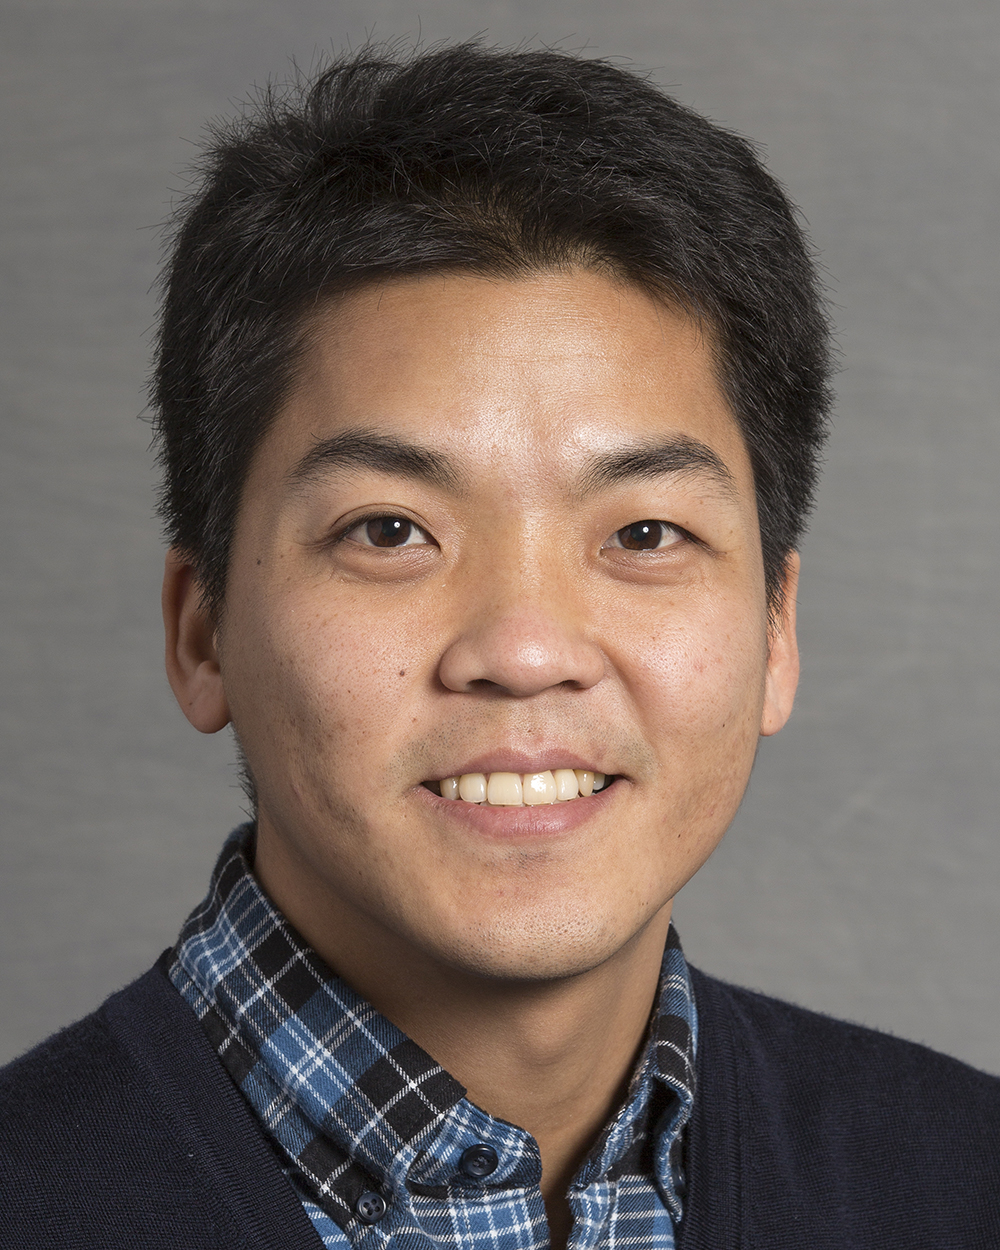
\includegraphics[width=1in,height=1.25in,clip,keepaspectratio]{cragkhit.jpg}}]{Chaiyong Ragkhitwetsagul}
is a lecturer at the Faculty of Information and Communication Technology, Mahidol University, Thailand. He received the PhD degree in Computer Science at University College London, where he was part of the Centre for Research on Evolution, Search, and Testing (CREST). His research interests include code search, code clone detection, software plagiarism, modern code review, and mining software repositories. %More info: \url{http://mucc.mahidol.ac.th/~chaiyong.rag}.
\end{IEEEbiography}
%\vspace{-1cm}

% % if you will not have a photo at all:
\begin{IEEEbiography}[{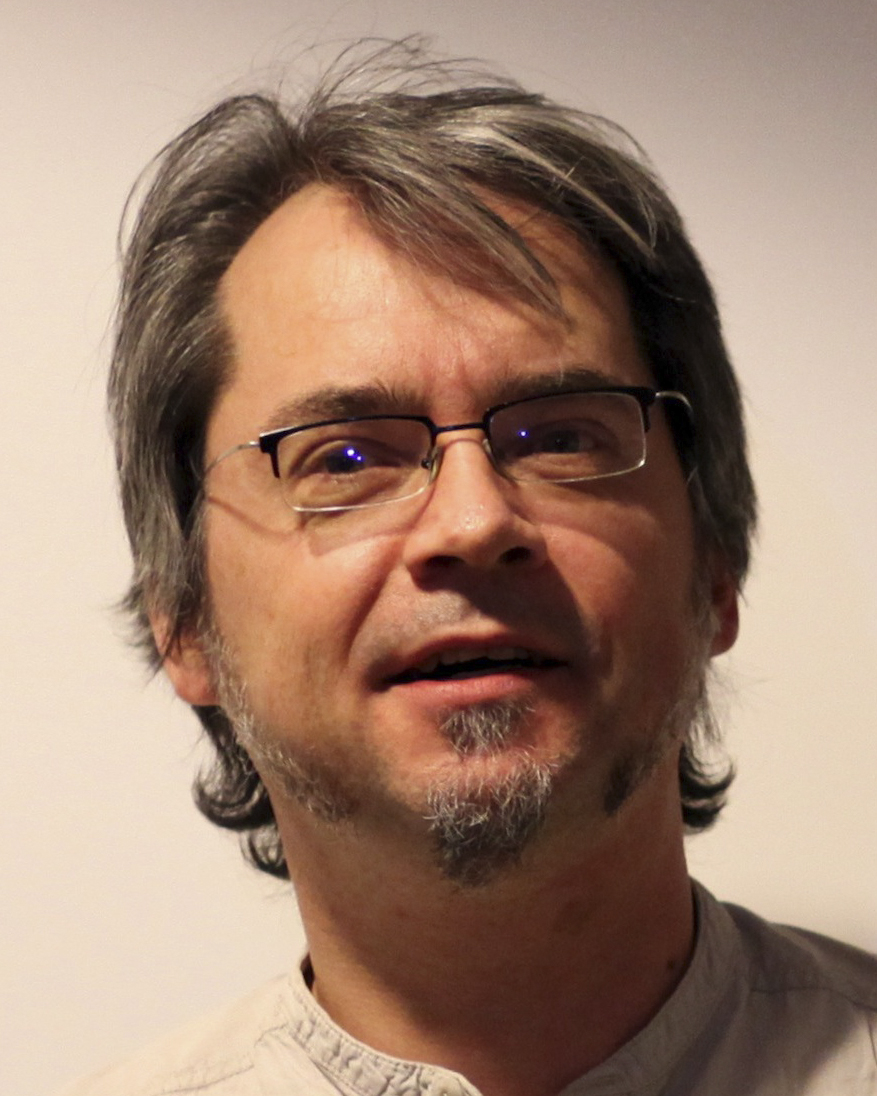
\includegraphics[width=1in,height=1.25in,clip,keepaspectratio]{jkrinke.jpg}}]{Jens Krinke}
is Associate Professor in the Software Systems Engineering
Group at the University College London, where he is Director of CREST,
the Centre for Research on Evolution, Search, and Testing.  His main
focus is software analysis for software engineering purposes. His
current research interests include software
similarity, modern code review, program analysis, and software testing.  He is well known for his work on
program slicing and clone detection.
\end{IEEEbiography}
%\vspace{-1cm}

\begin{IEEEbiography}[{
\includegraphics[width=1in,height=1.25in,clip,keepaspectratio]{mpaixao.png}}]{Matheus Paixao}
is currently a Research Assistant in the Computer Science Department at State University of Ceara. He recently received the PhD degree in Computer Science at University College London, where he was part of the Centre for Research on Evolution, Search, and Testing (CREST) and Software Systems Engineering (SSE) Group. He was supervised by Prof. Mark Harman and Dr. Jens Krinke. His research interests include software architecture, search-based software engineering, mining software repositories, modern code review and empirical software engineering.
\end{IEEEbiography}
%\vspace{-1cm}

\begin{IEEEbiography}[{
\includegraphics[width=1in,height=1.25in,clip,keepaspectratio]{giuseppe.png}}]{Giuseppe Bianco}
  received his bachelor degree in Computer Science from the University
  of Molise (Italy) under the supervision of Dr.~Rocco Oliveto. As
  part of an Erasmus+ traineeship, he spent three month at the
  CREST centre, University College London, UK, under the supervision
  of Dr.~Jens Krinke.~He is now a project manager at Corsi.it.
\end{IEEEbiography}
%\vspace{-0.5cm}

\begin{IEEEbiography}[{
\includegraphics[width=1in,height=1.25in,clip,keepaspectratio]{rocco.png}}]{Rocco Oliveto}
is Associate Professor at University of Molise (Italy), where he is
also the Director of the Computer Science Bachelor and Master programs
and the Director of the Software and Knowledge Engineering Lab (STAKE
Lab).
He is also one of the co-founders and CEO of DataSound, a spin-off of the University of Molise aiming at efficiently exploiting the priceless heritage that can be extracted from big data analysis via machine learning.
\end{IEEEbiography}
\vfill

% \begin{IEEEbiographynophoto}{Giuseppe Bianco}
% Biography text here.
% \end{IEEEbiographynophoto}

% % insert where needed to balance the two columns on the last page with
% % biographies
% %\newpage

% \begin{IEEEbiographynophoto}{Rocco Oliveto}
% Biography text here.
% \end{IEEEbiographynophoto}

% You can push biographies down or up by placing
% a \vfill before or after them. The appropriate
% use of \vfill depends on what kind of text is
% on the last page and whether or not the columns
% are being equalized.

%\vfill

% Can be used to pull up biographies so that the bottom of the last one
% is flush with the other column.
%\enlargethispage{-5in}



% that's all folks
\end{document}


